\documentclass[diploma]{softlab-thesis}

\usepackage{fontspec}
\usepackage{amsmath}
\usepackage{amsfonts}
\usepackage{algorithm}
\usepackage{algpseudocode}
\usepackage{pifont}
\usepackage{multirow}
\usepackage{array}
\usepackage{mdwlist}
\usepackage{subfig}
%\usepackage{floatrow}
%\usepackage{float}
\usepackage{verbatim}
\usepackage{color}
\usepackage{graphicx}
\usepackage{xunicode}
\usepackage{xltxtra}
\usepackage{url}
%\usepackage{dsfont}
%\usepackage{microtype}
\usepackage{hyphenat}
\usepackage{multicol}
\usepackage{wrapfig}
\usepackage{lipsum}
\usepackage{listings}
\usepackage{paralist}
\usepackage{ulem}
\usepackage{tocvsec2}
\usepackage[toc,page]{appendix}

%%%
%%%  The document
%%%

% FONT SETTINGS ===============================================================



\defaultfontfeatures{Mapping=tex-text}
\setromanfont{Times New Roman}

% CUSTOM COLORS ===============================================================

\definecolor{gray}{rgb}{0.5,0.5,0.5}
\definecolor{darkgreen}{rgb}{0.0,0.5,0.0}
\definecolor{mygreen}{rgb}{0,0.6,0}
\definecolor{mygray}{rgb}{0.5,0.5,0.5}
\definecolor{mymauve}{rgb}{0.58,0,0.82}
\definecolor{myorange}{RGB}{246,177,50}
\definecolor{myblue}{rgb}{0.13,0.13,1}
\definecolor{mybordo}{rgb}{0.37, 0.08, 0.25}  


% CUSTOM COMMANDS =============================================================
% FIGURE SETUP ===============================================================

\newcommand\diagram[2]{
	\begin{figure}[h!]
		\centering
		\includegraphics[width=\textwidth,height=\textheight,keepaspectratio]
		{diagrams/#2}
		\caption{#1}
		\label{fig:#2}
	\end{figure}
}

\newcommand\diagramscale[3]{
	\begin{figure}[h!]
		\centering
		\includegraphics[scale={#3}]
		{diagrams/#2}
		\caption{#1}
		\label{fig:#2}
	\end{figure}
}
\newcommand\diagramstrict[2]{
	\begin{figure}[H]
		\centering
		\includegraphics[keepaspectratio]
		{diagrams/#2}
		\caption{#1}
		\label{fig:#2}
	\end{figure}
}

\newcommand\fixme{\textrm{\textbf{\textcolor{red}{FIXME: }}}}
\newcommand\todo{\textrm{\textbf{\textcolor{myorange}{TODO: }}}}

\newtheorem{reliability}{Ορισμός 2 (Εμπιστοσύνη Αξιοπιστίας)}
\newtheorem{decision}{Ορισμός 3 (Εμπιστοσύνη Απόφασης)}
\newtheorem{soft_sec}{Ορισμός 1 (Soft Security)}
\newtheorem{reputation}{Ορισμός 4 (Φήμη)}




\lstset{
	backgroundcolor=\color{white},
	basicstyle=\small\ttfamily,		% style for code
	breakatwhitespace=false,        % sets if automatic breaks should only
 keywordstyle=\color{mybordo},
									% happen at whitespace
	breaklines=true,                % sets automatic line breaking
	captionpos=b,                   % sets the caption-position to bottom
	commentstyle=\color{mygreen},   % style for comments
	escapeinside={\%*}{*)},         % if you want to add LaTeX within your code
	frame=single,                   % adds a frame around the code
	keepspaces=true,                % keeps spaces in text, useful for 
	%keywordstyle=\color{blue}\bfseries,
					% keyword style
	numbers=left,
	numbersep=5pt,                  % how far the line-numbers are from the 
					% code
	numberstyle=\tiny\color{mygray},% style for line-numbers
	rulecolor=\color{black},
	stepnumber=1,                   % the step between two line-numbers. If 
					% it's 1, each line will be numbered
	stringstyle=\color{myblue},    % style for strings
	tabsize=2,                      % sets default tabsize to 2 spaces
}

% Define specific rules for each language

\lstdefinestyle{java}
{
	language=java
}

\newcommand\javacode[2]{
	\lstinputlisting[style=java, caption={#1}, label=lst:#2]{src/#2}
}

\usepackage[xetex,colorlinks=true,linkcolor=blue,citecolor=darkgreen]{hyperref}

\begin{document}

%%%  Title page

\frontmatter

\title{Κοινωνικός Αποκλεισμός και Επανένταξη Εικονικών Οντοτήτων στο Διαδίκτυο των Πραγμάτων} 

\author{Ελευθέριος Κόκορης - Κόγιας}
\authoren{Eleftherios Kokoris - Kogias}
\datedefense{03}{07}{2015}
\supervisor{Θεοδώρα Βαρβαρίγου}
\supervisorpos{Καθηγήτρια ΕΜΠ}
\committeeone{Θεοδώρα Βαρβαρίγου}
\committeeonepos{Καθηγήτρια ΕΜΠ}
\committeetwo{Βασίλειος Λούμος}
\committeetwopos{Καθηγητής Ε.Μ.Π.}
\committeethree{Δημήτριος Ασκούνης}
\committeethreepos{Αναπληρωτής Καθηγητής Ε.Μ.Π.}

\department{Τομέας Επικοινωνιών, Ηλεκτρονικής και Συστημάτων Πληροφορικής}

\maketitle
\def\templen{\parindent}
\setlength{\parindent}{0pt}
\setlength{\parskip}{2.0ex plus 0.5ex minus 0.2ex}
\begin{large}

\begin{abstractgr}
Στον 21ο αιώνα, ο ψηφιακός κόσμος έχει ενσωματωθεί στην καθημερινότητά μας. Έξυπνες συσκευές θα είναι σύντομα σε θέση να αποφασίζουν μόνες τους πώς θα ενεργήσουν ώστε να διευκολύνουν την ζωή μας.
Οι δράσεις αυτές θα πρέπει να βασίζονται στην χρήση γνώσης που αποκτήθηκε  από παρόμοιες συσκευές που αντιμετώπισαν    παρόμοια προβλήματα. Ωστόσο, καθώς αυτές οι συσκευές γίνονται όλο και ποιο αυτόνομες,
πιθανές επιθέσεις μπορεί να οδηγήσουν σε προβλήματα όχι μόνο στον ψηφιακό κόσμο αλλά και στον πραγματικό

Ο σκοπός της παρούσας διπλωματικής εργασίας είναι, ο σχεδιασμός και η υλοποίηση ενός decentralized συστήματος για την διαχείριση της εμπιστοσύνης των συσκευών μεταξύ τους στο πλαίσιο του
Κοινωνικού Διαδικτύου των Πραγμάτων (ΚΔτΠ)
 όπως αυτό απεικονίζεται από το project Cosmos .
 
Οι μέθοδοι διαχείρισης εμπιστοσύνης βασιζόμενη στη φήμη(reputation-based) έχουν χρησιμοποιηθεί με επιτυχία την προηγούμενη
δεκαετία κυρίως σε Peer-to-Peer συστήματα. Για το λόγο αυτό, η εργασία αυτή χτίστηκε επάνω σε 
state-of-the-art αλγορίθμους που χρησιμοποιούνται σε τέτοια συστήματα, με στόχο την περαιτέρω ανάπτυξη και τροποποίηση των
ιδεών ώστε να μπορούν να ενσωματωθούν στο πλαίσιο του Διαδικτύου των Πραγμάτων.
 
Αυτή η μελέτη προσδιορίζει τις πιθανές απειλές που μπορούν να προκύψουν στο ΚΔτΠ. Στην συνέχεια αναλύεται η προτεινόμενη αρχιτεκτονική του συστήματος διαχείρισης εμπιστοσύνης, η οποία είναι χτισμένη σε δύο παρατηρήσεις πάνω στης κοινωνικές αλληλεπιδράσεις των ανθρώπων.
 Πρώτον, όταν κάποιος θέλει να έχει πρόσβαση σε μια νέα υπηρεσία  ζητά προτάσεις από
τους φίλους του. Αυτή η διαδικασία χτίζει την φήμη (reputation) κάποιου. Δεύτερον, όταν κάποιος έχει αρκετές
αλληλεπιδράσεις με κάποιον άλλο, η φήμη δεν έχει σημασία πια. Εκεί έχει χτιστεί εμπιστοσύνη.
 
Μετά από κατάλληλη μοντελοποίηση αυτών των εννοιών χρησιμοποιώντας ιδέες από την Θεωρία των Πιθανοτήτων, προτείνετε το σύστημα RTIoT (Reputation \& Trust for the Internet of Things).Στην συνέχεια προστίθενται χαρακτηριστικά, όπως
η ικανότητα μίας κακόβουλης Εικονικής Οντότητας (ΕΟ) να εξιλεωθεί , η γρήγορη αναγνώριση 
αλλαγών στη συμπεριφορά των ΕΟ από αξιόπιστες σε κακόβουλες και η δυναμική ενσωμάτωση 
νέων ΕΟ στο σύστημα. Στο τέλος παρουσιάζουμε τα αποτελέσματα μέσα από μία προσομοίωση στο TRMSIM-WSN και τα συγκρίνουμε με άλλα συστήματα Εμπιστοσύνης/Φήμης.
	
    \begin{keywordsgr}
   εμπιστοσύνη, φήμη, ασφάλεια , Διαδίκτυο των πραγμάτων, Εικονική οντότητα, Cosmos, ασφάλεια κατανεμημένων συστημάτων, Κοινωνικό Διαδίκτυο των Πραγμάτων, κλιμάκωση
	\end{keywordsgr}
	
	
\end{abstractgr}

\begin{abstracten}
In the 21st century the digital world is incorporated on everyday life. Smart devices will soon be able to decide on their own of actions needed to be taken in order to facilitate our lives. 
These actions will be based on acquiring knowledge from similar devices that have encountered similar problems. However, as these devices are becoming autonomous, 
potential attacks can result in problems not only in the digital world but also in the physical one.  
 
The purpose of this thesis is the design and implementation of a decentralized system for Trust Management in the context of the ​
Social Internet of Things​
 as seen by the ​Cosmos​ project. 
 
Reputation-­based trust management methods have been successfully used in the  past 
decade mostly on Peer-­to-­Peer systems. For this reason, this study is built upon 
state-­of-­the-­art algorithms used on such systems, with the aim of further developing the 
ideas proposed and modifying them to fit the context of the Internet of Things. 
 
This study identifies the potential threats that can emerge in SIoT. After that the proposed 
architecture is analyzed. It is built upon two observations of the social interactions of humans.
 Firstly, when someone wants to access a new service he asks for referrals from 
his friends. This feedback is called Reputation. Secondly, when someone has enough 
interactions with someone else, the reputation does not matter any more. There has been built Trust. 
 
After appropriately modeling these notions using Probability Theory we propose the RTIoT(Reputation \& Trust for the Internet of Things) system. then we add features like 
the ability of a malicious Virtual Entity (VE) to get redemption, the quick identification of 
behavioural changes of VE’s from trustworthy to malicious and the dynamic integration of 
new VE’s in the system. In the end we demonstrate the results of a simulation using the TRMSIM-WSN simulator and compare them with other reputation systems. 

	\begin{keywordsen}
    Internet of Things, trust, reputation, scalability, security, Cosmos, Social Internet of Things, Distributed Systems security 
	\end{keywordsen}
\end{abstracten}

\begin{acknowledgementsgr}
===================================================================================

TODO

=============================================================================
\end{acknowledgementsgr}


\setlength{\parindent}{\templen}
\setlength{\parskip}{0pt}
\tableofcontents
\listoffigures
\listoftables
\renewcommand{\lstlistlistingname}{Κατάλογος Κώδικα}
\lstlistoflistings % changed the title above

\mainmatter
% moved these two commands here so that they don't influence the toc
\setlength{\parindent}{0pt}
\setlength{\parskip}{2.0ex plus 0.5ex minus 0.2ex}

\renewcommand\floatpagefraction{.7}

\chapter{Εισαγωγή}\label{ch:intro}

Όταν το 1969 γεννήθηκε το ARPANET η ιδέα που το ώθησε  ήταν η κοινή χρήση υπολογιστικών πόρων από απομακρυσμένες περιοχές. Δηλαδή εάν σε κάποιο ερευνητικό κέντρο χρειαζόταν να γίνουν πολλοί υπολογισμοί, να μπορούσαν να γίνουν σε κάποιο εξειδικευμένο υπολογιστικό σύστημα που ήταν γεωγραφικά απομακρυσμένο από το ερευνητικό κέντρο.

H ιδέα αυτή ποτέ δεν δούλεψε πραγματικά - για αρχή, όλοι οι υπολογιστές είχαν διαφορετικά λειτουργικά συστήματα και προγράμματα, ενώ η χρήση του μηχανήματος κάποιου άλλου ήταν πολύ δύσκολή. Επίσης μέχρι να υλοποιηθεί το ARPANET η τεχνολογία είχε φτάσει στο σημείο να μην το έχει ανάγκη αφού είχαν εμφανιστεί οι πρώτοι προσωπικοί υπολογιστές και ο καταμερισμός χρόνου σε υπολογιστικά συστήματα δεν πρόσφερε ποία τόσα οφέλη.

Έτσι είναι λογικό να πούμε ότι το ARPANET απέτυχε στο σκοπό του, αλλά στη διαδικασία αυτή έκανε μερικές σημαντικές ανακαλύψεις που είχαν ως αποτέλεσμα τη δημιουργία των τεχνολογιών του πρώτου Διαδικτύου. Σε αυτές περιλαμβάνονταν το e-mail, η μεταγωγή πακέτων εφαρμογών, και φυσικά η ανάπτυξη του (Transport Control Protocol - Internet Protocol) - Internet Protocol) ή TCP / IP.

Στην συνέχεια και λόγω της ραγδαίας εξάπλωσης των προσωπικών υπολογιστών το Internet έγινε ή ποίο μεγάλη απόδειξη της ισχύς του νόμου του Metclafe κατά τον οποίο:%\cite{Metclafe}
\begin{quotation}
"Η αξία ενός δικτύου είναι ανάλογη με το τετράγωνο του αριθμού των κόμβων, δηλαδή του αριθμού των χρηστών του δικτύου."
\end{quotation}

Σήμερα, το Διαδίκτυο με πάνω από 3 δισεκατομμύρια χρήστες είναι το βασικότερο μέσο 
εύρεσης και ανταλλαγής δεδομένων της ανθρωπότητας Ένας πολίτης του 21ου αιώνα δεν χρειάζεται να γνωρίζει κάθε μικρή πληροφορία, το μόνο που χρειάζεται να ξέρει είναι σε ποίο σημείο του διαδικτύου μπορεί να την βρει. Οπότε τώρα, βρισκόμαστε σε μία μεταβατική περίοδο. Το Διαδίκτυο είναι ευρέως αποδεκτό και αναγκαίο, αλλά η έμφυτη ανθρώπινη περιέργεια καθώς και η δημιουργικότητα μας οδηγούν στο επόμενο βήμα. Στο Διαδίκτυο των Πραγμάτων.

Ποία είναι όμως η διάφορα του Διαδικτύου από το Διαδίκτυο των Πραγμάτων; 

Τα λεγόμενα του Kevin Ashton, συνιδρυτή και εκτελεστικού διευθυντή του Auto-ID Center στο ΜΙΤ είναι ξεκάθαρα:%\cite{Ashton}
\begin{quotation}

"Σήμερα οι υπολογιστές - και, ως εκ τούτου, το Διαδίκτυο - εξαρτώνται σχεδόν εξ ολοκλήρου από τα ανθρώπινα όντα για πληροφορίες. Σχεδόν το σύνολο των περίπου 50 petabytes δεδομένων διαθέσιμων στο Διαδίκτυο, συλλαμβάνεται και δημιουργείται από τον άνθρωπο με την πληκτρολόγηση, το πάτημα ενός κουμπιού εγγραφής, την λήψη μιας ψηφιακής φωτογραφίας ή την σάρωση ενός barcode.


Το πρόβλημα είναι πώς, οι άνθρωποι έχουν περιορισμένο χρόνο, προσοχή και ακρίβεια. Γιαυτό και δεν είναι πολύ καλοί στο καταγραφή των δεδομένων που αφορούν τα πράγματα του γύρω κόσμου. Αν είχαμε υπολογιστές που ήξεραν οτιδήποτε μπορούσαν να ξέρουν για τα πράγματα γύρω τους - με τη χρήση δεδομένων που συνέλεξαν αυτόνομα χωρίς καμία βοήθεια από εμάς - τότε θα ήταν σε θέση να παρακολουθούν και να μετράνε τα πάντα. Έτσι θα μειωνόντουσαν σε μεγάλο βαθμό η σπατάλη αγαθών, οι απώλειες από λάθη και το γενικότερο κόστος. Θα γνωρίζαμε από το πότε τα πράγματα θα χρειάζονται αντικατάσταση ή επισκευή  έως και το αν ήταν φρέσκα ή όχι." 
\end{quotation}


\section{Κοινωνικό Διαδίκτυο των Πραγμάτων και Προβλήματα Εμπιστοσύνης}

Η Διπλωματική αυτή εργασία γεννήθηκε για να αντιμετωπισθούν ανησυχίες σχετικά με τις δράσεις των Εικονικών Οντοτήτων(Virtual Entities), οι οποίες αποτελούν την αναπαράσταση των πραγμάτων στον ψηφιακό κόσμο. Όταν λοιπόν σε αυτές τις Εικονικές Οντότητες προσθέσουμε την δυνατότητα να έχουν κοινωνικούς δεσμούς μέσο φιλίας, οικογένειας(ανήκουν στον ίδιο χρήστη) ή και ομοιότητας (έχουν τον ίδιο ρόλο στο σύστημα), τότε βρισκόμαστε στο Κοινωνικό Διαδίκτυο των Πραγμάτων \footnote{www.social-iot.org/}. Ειδικότερα αυτή η εργασία έγινε στα πλαίσια του COSMOS(Cultivate resilient smart Objects for Sustainable city applicatiOn) \footnote{www.iot-cosmos.eu/}, σκοπός του οποίου είναι η δημιουργία έξυπνων αντικειμένων, προκειμένου να καταστεί δυνατή μια έξυπνη πόλη. Στο COSMOS

\begin{itemize}
\item
Τα πράγματα θα είναι σε θέση να μάθουν βασιζόμενα σε εμπειρίες άλλον,
\item
 ενώ μέσα από την απόκτηση και την ανάλυση της γνώσης τα πράγματα θα γνωρίζουν τις συνθήκες και τα γεγονότα που συμβαίνουν και ανάλογα θα μεταβάλουν τη συμπεριφορά τους.
\item Οι διαχειριστικές αποφάσεις θα λαμβάνονται σε πραγματικό χρόνο για κάθε Εικονική Οντότητα βασιζόμενες στην ασφάλεια των πραγμάτων, την γεωγραφική τους θέση, τις σχέσεις που έχουν με άλλες εικονικές οντότητες καθώς και άλλες ψηφιακές πληροφορίες που θα εξάγονται από
\item Complex Event Processing και άλλες τεχνολογίες Κοινωνικών Mέσων ώστε να εντοπίζεται η χρήσιμη πληροφορία μεσα στον τεράστιο αριθμό δεδομένων (Big Data)
\end{itemize}


Στα πλαίσια λοιπόν του COSMOS  υπήρξε η ανάγκη να υπάρχει γνώση για το πόσο έμπιστος μπορεί να θεωρηθεί ένα πάροχος πληροφοριών ή/και υπηρεσιών. Με αυτή τη γνώση θα ήταν δυνατό: 
\begin{itemize}
	 \item Να εντοπίζεται γρήγορα η πιο αξιόπιστη πηγή πληροφοριών και να μειώνεται η επικοινωνία με ταυτόχρονη βελτιστοποίηση της απόδοσης
	 
 	 \item Να μπορεί μία Εικονική Οντότητα να κρίνει αυτόνομα πόσο πιθανό είναι να ικανοποιηθεί από μία προσφερόμενη υπηρεσία πριν προβεί στην δοσοληψία επειδή
 	 \begin{itemize}
 	 	\item μπορεί κάποια υπηρεσία να είναι προϊόν
 	 	\item μπορεί να μας δοθεί γνώση που θα ρισκάρει την ασφάλεια του συστήματος ή/και των τελικών χρηστών
 	 	\end{itemize}
\end{itemize}
 

\section{Δομή της Διπλωματική Εργασίας} 
Η διπλωματική εργασία δομείται ως εξής:

\begin{description}
\item[Chapter \ref{ch:bkg}] \hfill \\

BACKGROUND--TRUST + REPUTATION SYSTEMS+
PREVIOUS WORK (P2P/MOBILE-AD-HOC/IOT)
We provide all the necessary background information, both technical and
theoretical, so that the reader becomes familiar with the concepts and ideas
described. We cite a brief overview of the existing tracing and monitoring
infrastructures along with their advantages and disadvantages and how they
affected BlkKin's design and implementation. Finally, we describe Archipelago
and RADOS, the two systems we instrumented as a BlkKin's proof of concept.


\item[Chapter \ref{ch:dapper-zipkin}] \hfill \\
%%Vulneralibilities and attack-models
We describe the tracing concepts we employed in BlkKin so that we can achieve
the needed expressiveness. We so present Zipkin, which is an open-source
implementation of these tracing concepts and another BlkKin's building block.

\item[Chapter \ref{ch:design}] \hfill \\
%%%DESIGN + USE CASE SCENARIOS
We describe the BlkKin's design and architecture, the communication protocols
used and the tracing information flow.

\item[Chapter \ref{ch:implementation}] \hfill \\
%IMPLEMENTATION _WSN TOOLKIT
We analyze the process of creating BlkKin, our contributions to the tracing
infrastructure and the means used or created to extract the information needed
in order to serve the different roles that BlkKin can play.

\item[Chapter \ref{ch:evaluation}] \hfill \\
%EVALUATION
We cite our experience of using BlkKin in Archipelago and RADOS instrumentation
and its use as a debugging and an alerting mechanism.

%\item[Chapter \ref{ch:conclusion}] \hfill \\
CONCULSION-FUTURE WORK
We provide some concluding remarks and give some future work that could be done
to improve and evolve BlkKin.
\end{description}

\chapter{Θεωρητικό και Τεχνολογικό Υπόβαθρο}\label{ch:bkg}
\section{Ορισμοί Εννοιών}

Τα συστήματα εμπιστοσύνης και φήμης αποτελούν μία εξέλιξη της τελευταίας δεκαπενταετίας και χρησιμοποιούνται ευρέως σε διαδικτυακές αλληλεπιδράσεις μεταξύ τόσο ανθρώπων (e-bay, amazon) όσων και μηχανών (ευφυών δραστών, peer-to-peer συστημάτων κτλ.). Η ιδέα πάνω στην οποία βασίζονται είναι: η συλλογή κριτικής για έναν δράστη από άλλα μέλη της κοινότητας τα οποία έχουν ήδη αποκτήσει κάποιες εμπειρίες με τον πρώτο. Με αυτόν τον τρόπο υπάρχει η δυνατότητα να γνωρίζει κάποιος για "το ποιόν"  κάποιου άλλου χωρίς να χρειάζεται να τον γνωρίσει, δηλαδή να αλληλεπιδράσει με αυτόν. Αυτή η δυνατότητα με την σειρά της "εξαναγκάζει" του δράστες ενός συστήμηματος να συμμορφωθούν με τους κανόνες της δικτυακή κοινότητας της οποίας είναι μέλη.

Όταν η αίτηση για παροχή υπηρεσιών ή για απόκτηση δεδομένων γίνεται online μεταξύ οντοτήτων πρότερα αγνώστων μεταξύ τους τότε μπορούν να προκύψουν 2 βασικά προβλήματα.
\begin{enumerate}
\item Το πρώτο πρόβλημα που δεν εξετάζεται στην παρούσα εργασία είναι πώς τα δεδομένα που παρέχονται (και στην περίπτωση του COSMOS η γνώση) μπορεί να χρησιμοποιηθούν από τον παραλήπτη για διαφορετικούς σκοπούς από αυτούς που ισχυρίζεται. Έτσι να τον βοηθήσουμε άθελα μας στου κακόβουλους ή γενικότερα αντίθετους από το καλό της κοινότητας σκοπούς του.

\item Αντίθετα αυτή η εργασία εστιάζει στο πρόβλημα του ρίσκου πού παίρνει ένας χρήστης όταν ζητάει μία υπηρεσία, επειδή μπορεί τελικά να μην την λάβει σε ικανοποιητικό βαθμό οπότε να πρέπει να την ξαναζητήσει. Ακόμα είναι δυνατόν να κινδυνέψει η ασφάλεια του (αντί για σωστό αρχείο να σταλεί κάτι που περιέχει ένα Trojan), ενώ στην δική μας περίπτωση μπορεί η γνώση και εν συνεχεία οι δράσεις που προτείνονται να προκαλέσουν προβλήματα ασφαλείας όχι μόνο στον ψηφιακό κόσμο  των Εικονικών Οντοτήτων, όσο και στο φυσικό κόσμο των πραγμάτων και των ανθρώπων.
\end{enumerate}
\newpage
\subsection{Soft Security}


Ως ασφάλεια στην πιο γενική της έννοια μπορούμε να ορίσουμε "την κατάσταση στην οποία κάποιος ή κάτι βρίσκεται μακριά από οποιονδήποτε κίνδυνο και οποιαδήποτε προσπάθεια αλλοίωσης αυτής της κατάστασης θα αποτύχει" (ή και να πετύχει θα είναι δυνατή η επαναφορά στην αρχική κατάσταση χωρίς κόστος). Αυτός ο ορισμός είναι πολύ γενικός και περιλαμβάνει την ασφάλεια ανθρώπων την ασφάλεια περιουσιών ακόμα και την ασφάλεια υγείας.

Στην επιστήμη των υπολογιστών η βασικότερη κατηγορία ασφάλειας είναι η ασφάλεια που παρέχει ως υπηρεσία τον αποκλεισμό δραστών εξωτερικών του συστήματος από την απόκτηση πρόσβασης σε προστατευόμενες πληροφορίες ή πόρους. Αυτό το είδος "hard security" παρέχεται μέσα από την πιστοποίηση και τον έλεγχο πρόσβασης(access control) στα υπολογιστικά συστήματα καθώς και μέσα από την κρυπτογραφία στα κανάλια επικοινωνίας κατά την ανταλλαγή εμπιστευτικών πληροφοριών. Όμως το πρόβλημα μπορεί να αντιστραφεί και τότε όλες αυτές οι μέθοδοι είναι αναξιόπιστες. Αυτό θα συμβεί στην περίπτωση που η επίθεση γίνει εντός του συστήματος. Μία τέτοια επίθεση συμβαίνει όταν κάποιος δράστης ή γενικότερα κομμάτι του συστήματος, που έχει δικαίωμα να ενεργεί στο σύστημα, γίνει κακόβουλο ή ελαττωματικό. 

Αυτά τα προβλήματα λύνονται μέσα από εφαρμογές του "Soft Security" το οποίο είναι 

\begin{soft_sec}
Η συνεργασία των δραστών ενός συστήματος ώστε να αποκλείσουν μη κοινωνικά αποδεχτές συμπεριφορές. 
\end{soft_sec}

Με αυτόν τον τρόπο μπορεί να προστατευθεί η κοινότητα από κακόβουλους δράστες οι οποίοι όμως έχουν κάθε δικαίωμα να ενεργούν. Ουσιαστικά να εφαρμοστεί ένα είδος κοινωνικού αποκλεισμού. Ένας από τους βασικότερους μηχανισμούς για την επίτευξή αυτού του είδους ασφαλείας είναι με την χρήση των εννοιών της εμπιστοσύνης και της φήμης. \footnote{Φυσικά και η έννοια της εμπιστοσύνης είναι χρήσιμη και για το "hard security" (εμπιστοσύνη σε ένα πιστοποιητικό ή μία Certificate Authority που το υπογράφει), αλλά ουσιαστικά αυτό είναι μία εφαρμογή "Soft Security" της ανθρώπινης κοινωνίας που χρησιμεύει στο hard security της υπολογιστικής επιστήμης.} 



\subsection{Η Έννοια της Εμπιστοσύνης}

Στον κόσμο των ανθρώπινων οντοτήτων η ύπαρξη της έννοιας τις εμπιστοσύνης είναι εμφανής στις καθημερινές μας αλληλεπιδράσεις. Θα μιλήσουμε για τα προβλήματα μας και της εμπειρίες μας -δηλαδή θα δώσουμε ευαίσθητες προσωπικές πληροφορίες- στους φίλους μας οι οποίοι περιμένουμε να μας βοηθήσουνε με δικές τους εμπειρίες, καθώς και να βοηθηθούν από τις πληροφορίες μας. Επίσης θα πάμε να αγοράσουμε προϊόντα από μαγαζιά που γνωρίζουμε και έχουμε ξαναπάει επειδή πιστεύουμε πως η ποιότητα ου προϊόντος ή της υπηρεσίας που θα λάβουμε θα είναι ικανοποιητική για εμάς.

Στον κόσμο όμως της υπολογιστικής επιστήμης ο ορισμός και η μοντελοποίηση της εμπιστοσύνης είναι αρκετά δύσκολη. Αυτό συμβαίνει επειδή τις ανθρώπινες σχέσεις τις κυβερνούνε συναισθήματα όπως αγάπη και αφοσίωση που δεν έχουν καμία θέση στον ψηφιακό κόσμο. Στο έργο του Audun Jøsang %\cite survey trust josang
υπάρχει μία εξαιρετική συγκέντρωση για τους διαφόρους ορισμούς της εμπιστοσύνης και τις φήμης.
Εκεί λοιπόν αναφέρεται πώς υπάρχουν δύο βασικοί ορισμοί για την εμπιστοσύνη τους οποίους ονομάζουμε εμπιστοσύνη αξιοπιστίας (reliability trust) και εμπιστοσύνη απόφασης (decision trust)


Όπως προϊδεάζει και το όνομα η εμπιστοσύνη αξιοπιστίας μπορεί να ερμηνευθεί ως η αξιοπιστία κάποιου δράστη ή αντικειμένου, και ο ορισμός του Gambetta %\cite gambetta apo josang
 παρέχει ένα παράδειγμα του πώς μπορεί να διατυπωθεί:
\begin{reliability}
Εμπιστοσύνη είναι η υποκειμενική πιθανότητα από την οποία ένα άτομο, Α, περιμένει από ένα άλλο άτομο, Β, να κάνει μία συγκεκριμένη ενέργεια από την οποία εξαρτάται η ευημερία του.
\end{reliability}

Αυτός ορισμός περιεχέι την έννοια της εξάρτησης του Α από τον Β, και την αξιοπιστία (δηλαδή την πιθανότητα) του Β όπως την αντιλαμβάνεται ο Α.

Όμως η εμπιστοσύνη μπορεί να είναι πολύ πιο σύνθετη από τον παραπάνω ορισμό. Αυτό συμβαίνει επειδή το γεγονός ότι η αξιοπιστία ενός δράστη είναι υψηλή δεν οδηγεί στην τυφλή εμπιστοσύνη του για οποιαδήποτε ενέργεια. Το ρίσκο τις αποτυχίας μίας συγκεκριμένη συναλλαγής μπορεί να είναι πολύ μεγάλο. Δηλαδή με απλά λόγια, ένας δράστης μπορεί να θεωρηθεί αξιόπιστος για μία απλή συναλλαγή, όμως για κάποια πιο κρίσιμη η αξιοπιστία του να μην είναι αρκετά καθησυχαστική. Για να συμπεριλάβουμε λοιπόν την πιο ευρεία έννοια που μπορεί να χαρακτηριστεί ως εμπιστοσύνη, μπορεί να χρησιμοποιηθεί ο ακόλουθος ορισμός των  McKnight \& Chervany %\cite mcknight apo josang

\begin{decision}
Η εμπιστοσύνη είναι ο βαθμός στον οποίο ένα άτομο είναι πρόθυμο να εξαρτηθεί από κάτι ή κάποιον σε μια δεδομένη κατάσταση με ένα αίσθημα σχετικής ασφάλειας, ακόμη και αν οι αρνητικές συνέπειες είναι δυνατές.
\end{decision}

Ο γενικότερος αυτός ορισμός μας παρέχει μία χρήσιμη ασάφεια αφού περιλαμβάνει πτυχές μίας ευρύτερης έννοιας της εμπιστοσύνης, η οποία περιέχει της έννοιες της εξάρτησης από αυτόν που απολαμβάνει την εμπιστοσύνη, της αξιοπιστίας αυτού καθώς και της ύπαρξης ενός παράγοντα κινδύνου που πρέπει να αποδεχτεί το άτομο που καλείτε να εμπιστευτεί κάποιο άλλο άτομο, ανάλογο με την εκάστοτε συναλλαγή.

\subsection{Η Έννοια της Φήμης}

Γυρίζοντας πίσω στον κόσμο τον ανθρώπων μπορούμε εύκολα να εντοπίσουμε άλλη μία έννοια η οποία χαρακτηρίζει εάν μεγάλο αριθμό ενεργειών και αποφάσεων μας. Αυτή η έννοια είναι η φήμη. Όταν για παράδειγμα θέλει ένα άτομο να αποκτήσει πρόσβαση σε μία υπηρεσία καινούργια (δηλαδή που δεν την έχει ξαναχρησιμοποιήσει), όπως για παράδειγμα να πάει σε ένα φροντιστήριο το παιδί του να μάθει μία ξένη γλώσσα ή να βρει έναν καλό μηχανικό για να του χτίσει το σπίτι του. Τότε ένα από τους βασικούς παράγοντες της επιλογής θα είναι η φήμη. Δηλαδή θα συλλέξει πληροφορίες από τον κοινωνικό του περίγυρο και αφού τις σταθμίσει ανάλογα με την εμπιστοσύνη του στης πηγές προέλευσής τους θα εξάγει την φήμη του πιθανού παρόχου της υπηρεσίας.
\newpage

Στην Υπολογιστική Επιστήμη μοντελοποιούμε την φήμη με ακριβώς τον ίδιο τρόπο. Έτσι μπορούμε να ορίσουμε την φήμη ως:
\begin{reputation}
Φήμη είναι το τι λέγεται ή πιστεύεται δημόσια για το ποιόν ή τον χαρακτήρα κάποιου ατόμου ή αντικειμένου
\end{reputation}

Παρ'όλη την στενή συγγένεια των εννοιών της φήμης και της εμπιστοσύνης, έχουν μία θεμελιώδη διαφορά. Η φήμη βασίζεται στην εμπειρία του κοινωνικού συνόλου με ένα άτομο ενώ η εμπιστοσύνη είναι προσωπικό ζήτημα και δεν επηρεάζεται από το κοινωνικό σύνολο. Μπορούμε να δούμε ξεκάθαρα την διαφορά τους στης παρακάτω προτάσεις:
\begin{enumerate}
\item \begin{quote} 
"Θα εμπιστευτώ τον Χ επειδή έχει καλή φήμη"
\end{quote}
\item \begin{quote}
 "Θα εμπιστευτώ τον Υ παρόλο που έχει κακή φήμη, επειδή μαζί μου είναι καλός"
\end{quote}
\end{enumerate}

Οι παραπάνω φράσεις δείχνουν ξεκάθαρα πώς παρόλο που η υπηρεσία που τα δυο άτομα θέλουν αιτηθούν είναι η ίδια, το άτομο 1, που δεν έχει αλληλεπιδράσει ποτέ με τον Υ, θα προτιμήσει τον Χ εμπιστευόμενος το κοινωνικό σύνολο από όπου εξήγε την καλή φήμη του Χ. Αντίθετα το άτομο 2 ένα και ξέρει πως ο Χ έχει καλύτερη φήμη από τον Υ θα διαλέξει τον Υ επειδή έχει καλή προϊστορία μαζί του, ουσιαστικά επειδή τον εμπιστεύεται. Αυτή η παρατήρηση δείχνει πώς η υποκειμενική γνώμη ενός ατόμου για ένα άλλο έχει μεγαλύτερο βάρος από την γνώμη του κοινωνικού σύνολου και έτσι στο τέλος η εμπιστοσύνη σε ένα άτομο θα υπερισχύσει της φήμης του.

\section{Αρχιτεκτονικές Δικτύωσης Συστημάτων Εμπιστοσύνης}

Όπως αναφέραμε οι κλασσικοί τρόποι που έχει η κοινωνία για την εξαγωγή φήμης και εμπιστοσύνης απουσιάζουν από τα online συστήματα που κατασκευάζουμε. Για αυτό τον λόγο χρειαζόμαστε ηλεκτρονικά υποκατάστατα. Οι βασικότερες ιδιότητες που πρέπει να έχει ένα ένα σύστημα βασιζόμενο στην φήμη είνα: %\citep{Resnick} απο το ίδιο

\begin{enumerate}
\item Οι οντότητες πρέπει να είναι μακρόβιες έτσι ώστε μετά από μία συναλλαγή να υπάρχει πιθανότητα μία μελλοντικής επαφής με την ίδια οντότητα

\item Οι συναλλαγές να αποτιμώνται και οι βαθμολογίες να διανέμονται σε άλλα μέλη τις κοινότητας

\item Οι αποφάσεις για της συναλλαγές μίας οντότητας να επηρεάζονται από τις βαθμολογίες των παλιών συναλλαγών
\end{enumerate}

Οι τεχνικές αρχές για τα συστήματα φήμης περιγράφονται στο παρών και το ακόλουθο τμήμα. Η αρχιτεκτονική του δικτύου καθορίζει πώς οι αξιολογήσεις των συναλλαγών αξιοποιούνται και διανέμονται ανάμεσα στα μέλη των συστημάτων. Οι δύο κύριοι τύποι είναι οι συγκεντρωτικές και οι κατανεμημένες αρχιτεκτονικές.%\cite pali ton josang
\subsection{Συγκεντρωτικές Αρχιτεκτονικές}

Στις συγκεντρωτικές αρχιτεκτονικές, οι πληροφορίες για την επίδοση ενός μέλους συγκεντρώνονται από τις βαθμολογίες των άλλων μελών της κοινότητας οι οποίοι είχαν άμεση εμπειρία με τον πρώτο. Η κεντρική αρχή η οποία συγκεντρώνει τις βαθμολογίες εξάγει τελικά την δείκτη της φήμης του κάθε μέλους της κοινότητας τον οποίο μπορεί να δει όποιος ενδιαφέρεται. Τα άλλα μέλη με την σειρά του χρησιμοποιούν αυτούς τους δείκτες όταν θέλουν να αλληλεπιδράσουν με άγνωστα, για αυτούς, μέλη της κοινότητας και θέλουν να αποφασίσουν εάν θα προβούν σε κάποια συναλλαγή ή όχι. Η ουσία είναι πώς συναλλαγές με άτομα που έχουνε υψηλότερο δείκτη φήμης έχουν πιο πολλές πιθανότητες να είναι επιτυχημένες από συναλλαγές με άτομα χαμηλού δείκτη φήμης.

Στο Σχ.\ref{fig:centralized.png} παρακάτω φαίνεται μία τυπική αρχιτεκτονική με κεντρική αρχή.

%
\diagramscale{Συγκεντρωτική Αρχιτεκτονική}{centralized.png}{0.9}

Ο Α θέλει να προβεί σε μία συναλλαγή με τον Β, ενώ δεν έχει κάποια παρελθοντική εμπειρία με αυτόν. Για αυτό ρωτάει την κεντρική αρχή, η οποία με την σειρά της γυρίζει τον δείκτη φήμης που έχει υπολογίσει βασιζόμενη σε πληροφορίες από άλλα μέλη τις κοινότητας όταν αυτά αλληλεπίδρασαν με τον Β και κοινοποίησαν στην κεντρική αρχή την εμπειρία τους.

Τα δύο βασικά κομμάτια των συγκεντρωτικών συστημάτων φήμης είναι:
\begin{enumerate}

\item Tα συγκεντρωτικά πρωτόκολλα επικοινωνίας που επιτρέπουν στους συμμετέχοντες να παρέχουν αξιολογήσεις για τα μέλη των συναλλαγών στην κεντρική αρχή, καθώς και να αποκτήσουν έναν δείκτη φήμης των πιθανών εταίρων στην συναλλαγή από την κεντρική εξουσία.

\item Έναν τρόπο υπολογισμού φήμης που χρησιμοποιείται από την κεντρική αρχή να εξάγει δείκτες φήμη για κάθε μέλος, με βάση τις αξιολογήσεις που έλαβε, και ενδεχομένως άλλες πληροφορίες όπως θα δούμε στην παράγραφο \ref{sec:compute} παρακάτω.

\end{enumerate}
\newpage
\subsection{Κατανεμημένες Αρχιτεκτονικές}

Υπάρχουν περιβάλλοντα όπου ένα κατανεμημένο σύστημα φήμης, δηλαδή χωρίς τις κεντρικές λειτουργίες, είναι καταλληλότερο από ένα συγκεντρωτικό σύστημα. Σε ένα κατανεμημένο σύστημα, δεν υπάρχει κεντρικό σημείο για την υποβολή των αξιολογήσεων ή την απόκτηση δεικτών φήμης των άλλων. Αντ'αυτού, μπορεί να υπάρχουν κατανεμημένα σημεία αποθήκευσης όπου μπορούν να υποβληθούν αξιολογήσεις ή ο κάθε συμμετέχοντας απλά να καταγράφει τη γνώμη του σχετικά με τις εμπειρίες του με άλλα μέλη της κοινότητας, και να παρέχει ο ίδιο τις πληροφορίες αυτές, κατόπιν αιτήματος. Ένας τρίτος συμβαλλόμενος, ο οποίος ενδιαφέρεται να συναλλαχθεί με δεδομένο άλλο μέλος της κοινότητας, πρέπει να βρει τις κατανεμημένες αποθήκες, ή να προσπαθήσει να αποκτήσει βαθμολογίες από όσα μέλη της κοινότητας μπορεί τα οποία είχαν άμεση εμπειρία με το εν λόγω μέλος-στόχο. Αυτό απεικονίζεται στο Σχ.\ref{fig:distributed.png}  παρακάτω.

\diagramscale{Κατανεμημένη Αρχιτεκτονική}{distributed.png}{0.9}

Ο τρίτος συμβαλλόμενος (στο Σχ.\ref{fig:distributed.png}  ο Α) υπολογίζει μόνος του των δείκτη της φήμης του μέλους στόχου (Β) βασιζόμενος στην μερική ή ολική γνώση που συνέλεξες από ένα τους "γνωστούς" του. (εδώ έχει μερική γνώση επειδή δεν πήρε feedbacκ από τον Δ).

Τα δύο βασικά κομμάτια των κατανεμημένων συστημάτων φήμης είναι:
\begin{enumerate}

\item Tα κατανεμημένα πρωτόκολλα επικοινωνίας που επιτρέπουν στους συμμετέχοντες να λάβουν και να στείλουν βαθμολογίες για άλλα μέλη της κοινότητας

\item Έναν τρόπο υπολογισμού φήμης που χρησιμοποιείται από κάθε μέλος της κοινότητας για να εξάγει δείκτες φήμης με βάση τις αξιολογήσεις που έλαβε, και ενδεχομένως άλλες πληροφορίες όπως θα δούμε στην παράγραφο \ref{sec:compute} παρακάτω.

\end{enumerate}
\newpage
\section{Τρόποι υπολογισμοί φήμης και εμπιστοσύνης}\label{sec:compute}

\subsection{Bayesian}

Τα Bayesian συστήματα λαμβάνουν δυαδικές αξιολογήσεις ως είσοδο (δηλαδή θετική ή αρνητική τιμή), και βασίζονται στον υπολογισμό των δεικτών  με χρήση των \textit{βήτα συναρτήσεων πυκνότητας πιθανότητας} (ΣΠΠ). Ο  ενημερωμένος δείκτης υπολογίζεται συνδυάζοντας τις προηγούμενες τιμές των δεικτών φήμης με τη νέα βαθμολόγια.%\cite apo johang [31,49-51,68].
 Ο δείκτης της φήμης ή/και της εμπιστοσύνης μπορεί να αναπαρασταθεί είτε με τη μορφή μιας πλειάδας παραμέτρων βήτα μορφής \textit{(α, β)} (όπου \textit{α} και \textit{β} αντιπροσωπεύουν τον αριθμό των θετικών και αρνητικών αξιολογήσεων, αντίστοιχα), είτε με τη μορφή της τιμής της προσδοκία της βήτα ΣΠΠ. Προαιρετικά μπορεί να υπάρχει και ή διακύμανση. Το πλεονέκτημα των Bayesian συστημάτων είναι ότι παρέχουν μία θεωρητικά ορθή βάση για τον υπολογισμό των δεικτών, ενώ το μόνο μειονέκτημα που θα μπορούσε να καταλογιστεί είναι ότι είναι υπερβολικά πολύπλοκα για να τα κατανοήσει ο μέσος άνθρωπος.

Η βήτα οικογένεια κατανομών είναι μια συνεχής οικογένεια συναρτήσεων κατανομής μεταβαλλόμενη από τις δύο παραμέτρους α και β. Η βήτα ΣΣΠ συμβολίζεται με beta(p | α, β) μπορεί να εκφραστεί χρησιμοποιώντας τη συνάρτηση γάμμα Γ ως εξής:
\begin{equation}
beta(p|\alpha,\beta)= \frac{\Gamma\left(\alpha + \beta\right)}{\Gamma\left(\alpha\right)\Gamma\left(\beta\right)}p^{\alpha−1}\left(1-p\right)^{\beta-1} o \pi o \upsilon\ \  0\  ≤\  p\  ≤\  1,\  \alpha,\  \beta\  >\  0
\label{eq:beta}
\end{equation}

με τον περιορισμό ότι η πιθανότητα $ p \neq 0 \ \  \alpha \nu \  \alpha \  <\ 1,$ και $ p \neq 1 \ \  \alpha \nu \  \beta \  <\ 1$.
Η τιμή της προσδοκίας της κατανομής beta δίνεται από:

\begin{equation}
E\left(p\right) = \frac{\alpha}{\left(\alpha+\beta\right)}
\label{eq:exp}
\end{equation}

Στην αρχική κατάσταση όπου δεν είναι τίποτα γνωστό η εκ των προτέρων ΣΠΠ είναι η ομοιόμορφη κατανομή βήτα κατανομή όπου $\alpha=1,\ \beta = 1$ η οποία φαίνεται στο σχήμα \ref{fig:beta.png}  παρακάτω. Στην συνέχεια αφού παρατηρηθούν ν θετικές και μ αρνητικές βαθμολογίες η εξαγόμενη κατανομή είναι η βήτα κατανομή(α,β) όπου α=ν+1 και β=μ+1. Για παράδειγμα εάν παρατηρηθούν 7 θετικές και 1 αρνητική βαθμολογίες τότε η ΣΠΠ φαίνεται στο σχήμα \ref{fig:beta.png} .


\diagramscale{Βήτα Συναρτήσεις Πυκνότητας Πιθανότητας}{beta.png}{0.4}
Μία ΣΠΠ αυτού του τύπου εκφράζει την αβέβαιη πιθανότητα ότι οι μελλοντικές αλληλεπιδράσεις θα είναι θετικές. Το πιο φυσικό είναι να καθοριστεί ο δείκτης φήμης ως συνάρτηση της τιμής της προσδοκίας. Η τιμή αυτή (της πιθανότητας προσδοκίας) σύμφωνα με την Εξ. \ref{eq:exp} είναι Ε(p) = 0,8. Αυτό μπορεί να ερμηνευθεί λέγοντας ότι η σχετική συχνότητα μιας θετικής έκβασης στο μέλλον είναι αβέβαιη, και ότι ή πιθανότερη τιμή της (της συχνότητας) είναι 0,8.

\subsection{ Διακριτών Καταστάσεων}

Οι άνθρωποι μπορούν συχνά να αξιολογήσουν καλύτερα την απόδοση συστημάτων όταν οι τιμές έχουν διακριτή λεκτική μορφή, σε σχέση με όταν είναι συνεχείς μετρήσεις. Αυτό ισχύει επίσης και για τον καθορισμό των δεικτών εμπιστοσύνης. Ορισμένοι συγγραφείς, συμπεριλαμβανομένων %\cite[1,8,9,44],
 έχουν προτείνει διακριτά μοντέλα εμπιστοσύνης. Για παράδειγμα, στο μοντέλο του Αμπντούλ Ραχμάν \& Hailes (2000) %\cite[1]
 , η αξιοπιστία ενός παράγοντα Χ μπορεί να έχει τιμές:
Πολύ Αξιόπιστη, Αξιόπιστη, Αναξιόπιστη, Πολύ Αναξιόπιστη
Το μέλος της κοινότητας (Υ) που θέλει να βρει την αξιοπιστία κάποιου μπορεί να συνδυάσει τη δική του άποψη  για την αξιοπιστία του Χ με την φήμη που εξάγει από την κοινότητα.
 
Look-up πίνακες, με εγγραφές για την υποβάθμιση / αναβάθμιση της εμπιστοσύνης που έχει ο Υ στον Χ, χρησιμοποιούνται για να καθορίσουν την εξαγόμενη εμπιστοσύνη στο Χ. Κάθε φορά που ο Υ είχε προσωπική εμπειρία με το Χ, αυτό μπορεί να χρησιμοποιηθεί για τον προσδιορισμό τής αξιοπιστίας του. Η υπόθεση είναι ότι η προσωπική εμπειρία αντικατοπτρίζει την πραγματική αξιοπιστία του Χ και ότι η φήμη που λαμβάνει για τον Χ, η οποία διαφέρει από την προσωπική εμπειρία, δείχνει αν ο Υ υποτιμά ή υπερτιμά τον Χ. Παρατηρήσεις από "φίλους" που υπερεκτιμούν των Υ θα υποβαθμιστεί πριν ληφθούν υπόψιν, και το αντίστροφο.

Το μειονέκτημα των διακριτών τιμών είναι ότι δεν είναι εύκολο να εφαρμοστούν σε αυτά κλασσικοί υπολογισμοί. Αντ 'αυτού, πρέπει να χρησιμοποιηθούν ευριστικοί μηχανισμοί όπως look-up πίνακες.

\subsection{Ασαφούς Λογικής}

Η εμπιστοσύνη και η φήμη μπορούν να παρασταθούν ως γλωσσικά ασαφείς έννοιες, όπου συναρτήσεις συμμετοχής περιγράφουν σε ποιο βαθμό ένας παράγοντας μπορεί να περιγραφεί ως π.χ. αξιόπιστος ή αναξιόπιστες. Η ασαφής λογική προβλέπει κανόνες για το συλλογισμό με ασαφείς μετρικές αυτού του είδους. Το σύστημα που προτείνει Manchala (1988%\cite [44]
,καθώς και η εξαγωγή τής φήμη στο συστήματος REGRET που προτείνουν οί Sabater \& Sierra (2001,2002) %\cite [59-61]
 εμπίπτουν σε αυτή την κατηγορία. Στο σύστημα των Sabater \& Sierra, αυτό που αποκαλούν ατομική φήμη προέρχεται από ιδιωτικές πληροφορίες σχετικά με ένα συγκεκριμένο δράστη ενώ αυτό που ονομάζουν κοινωνική φήμη προέρχεται από την ενημέρωση του κοινού σχετικά με αυτόν τον δράστη, τέλος αυτό που αποκαλούν context dependent φήμη εξάγεται από τις συμφραζόμενες πληροφορίες.

\subsection{Ροής Εμπιστοσύνης}

Τα συστήματα που υπολογίζουν την εμπιστοσύνη ή τη φήμη με επανάληψη μέσω βρόχου ή με αυθαίρετα μεγάλες αλυσίδες μπορούν να ονομαστούν μοντέλα ροής.

Ορισμένα μοντέλα ροής έχουν σταθερή τιμή ολικής εμπιστοσύνης / φήμης για το σύνολο του συστήματος και η τιμή αυτή μπορεί να κατανεμηθεί μεταξύ των μελών της κοινότητας. Οι συμμετέχοντες μπορούν να αυξήσουν την εμπιστοσύνη / φήμη τους μόνο σε βάρος των άλλων. Ό PageRank της Google [52] ανήκει σε αυτή την κατηγορία. Σε γενικές γραμμές, η φήμη ενός συμμετέχοντος αυξάνει ως συνάρτηση της εισερχόμενης ροής, και μειώνεται ως συνάρτηση της εξερχόμενης ροής. Στην περίπτωση της Google, πολλοί υπερσύνδεσμοι εισερχόμενοι (που δείχνουν σε αυτή) σε μια ιστοσελίδα συμβάλλουν στην αύξηση του δείκτη PageRank ενώ πολλοί υπερσύνδεσμοι εξερχόμενοι (που υπάρχουν μέσα) από μια ιστοσελίδα οδηγούν στη μείωση του δείκτη PageRank για την εν λόγω ιστοσελίδα.

Τα μοντέλα ροής δεν απαιτούν πάντα το άθροισμα των βαθμολογιών φήμης / εμπιστοσύνης να είναι σταθερό. Ένα τέτοιο παράδειγμα είναι το σύστημα EigenTrust [35], το οποία υπολογίζει δείκτες εμπιστοσύνη σε δίκτυα P2P μέσω επαναλαμβανόμενου πολλαπλασιασμού και  ομαδοποίησης των βαθμολογιών εμπιστοσύνης έως ότου οι δείκτες εμπιστοσύνης για όλα τα μέλη της P2P κοινότητας συγκλίνουν σε σταθερές τιμές.

\subsection{Άθροιση ή εξαγωγή Μέσου Όρου}

Η συνηθέστερη μορφή υπολογισμού φήμης / εμπιστοσύνης είναι να υπολογίζεται το συνολικό αριθμό των θετικών αξιολογήσεων και το συνολικό αριθμό των αρνητικών αξιολογήσεις ξεχωριστά, και να εξάγετε μια συνολική βαθμολογία ως το θετικό άθροισμα μείον το αρνητικό. Αυτή είναι η αρχή που χρησιμοποιείται στο φόρουμ του eBay η οποία περιγράφεται λεπτομερώς στο [55]. Το πλεονέκτημα είναι ότι ο καθένας μπορεί να καταλάβει την αρχή πίσω τον υπολογισμό της φήμη, το μειονέκτημα είναι ότι ο υπολογισμός είναι πρωτόγονος και, ως εκ τούτου ο δείκτης της φήμης δίνει μιας φτωχής εικόνα αν και αυτό οφείλεται επίσης στον τρόπο που παρέχεται αξιολόγηση.

Ένα ελαφρώς πιο προχωρημένο σύστημα που προτείνεται στο π.χ. [63] είναι να υπολογιστεί ο δείκτης της φήμη ως ο μέσος όρος όλων των αξιολογήσεων. Η αρχή αυτή χρησιμοποιείται στα συστήματα φήμης πολλών εμπορικές ιστοσελίδων, όπως  της Amazon περιγράφεται στο \ref{sec:prev}

Προηγμένα μοντέλα σε αυτή την κατηγορία υπολογίζουν ένα σταθμισμένο μέσο όρο όλων των αξιολογήσεων, όπου το βάρος της αξιολόγησης μπορεί να καθορίζεται από παράγοντες όπως ο εκτιμητής της αξιοπιστίας / φήμη, τη ηλικία της αξιολόγησης, η σχέση μεταξύ αξιολογητή και αξιολογούμενου κ.λ.π. Το σύστημα που παρουσιάζεται στην υπόλοιπη εργασία εμπίπτει σε αυτήν την κατηγορία.
\newpage
\section{Γνωστά Συστήματα φήμης κ εμπιστοσύνης σε διαφόρους τομείς}\label{sec:prev}

Τα συστήματα φήμης και εμπιστοσύνης είναι ευρέως διαδεδομένα σε πολλούς τομείς όπου χρησιμοποιούνται πληροφοριακά συστήματα. Ο βασικός λόγος που εφαρμόζεται ένα σύστημα φήμης-εμπιστοσύνης είναι για να αντιμετωπίσει κακόβουλους συμμετέχοντες σε μία κοινότητα οντοτήτων και έτσι να βελτιωθεί τόσο η ασφάλεια όσο και η ποιότητα των υπηρεσιών.

\subsection{Business}

\subsubsection{E-bay}

\subsubsection{Amazon}

\subsubsection{PageRank}

\subsection{Mobile-ad-hoc Networks}

\subsubsection{Le Boudec}

\subsubsection{hubeaux}

\subsubsection{stanford}

\subsection{Peer-to-Peer Systems}

\subsubsection{EingenTrust}

\subsubsection{PeerTrust}

\subsubsection{PowerTrust}

\subsection{Internet of Things}

\subsubsection{Atzori}



\chapter{Τύποι επιθέσεων - Αντιμετώπιση με RT-IOT}\label{ch:design}

\section{Επιθέσεις στο Διαδίκτυο των πραγμάτων}

Όπως αναφέρθηκε στο Κεφάλαιο \ref{ch:bkg} ένας από τους κινδύνους παραβίασης της ασφάλειας του Κοινωνικού Διαδικτύου των Πραγμάτων πηγάζει από επιθέσεις κακόβουλων οντοτήτων οι οποίες όμως νομίμως δρουν εντός της κοινωνίας των πραγμάτων. Σε αυτό το κομμάτι του κεφαλαίου θα αναλύσουμε τις βασικότερες επιθέσεις που μπορούν να συμβούν.

\subsection{Μεμονωμένες κακόβουλες Εικονικές Οντότητες}\label{sec:indv}

Οι μεμονωμένες κακόβουλες Εικονικές Οντότητες Σχ.\ref{fig:individual.png} είναι o απλούστερος και ο βασικότερος τύπος επίθεσης. Σε αυτήν την περίπτωση ένα ποσοστό των μελών της κοινότητας έχοντας κακόβουλους σκοπούς προσπαθούν να εκμεταλλευτούν την εμπιστοσύνη των υπόλοιπων και όταν τους ζητηθεί κάποια υπηρεσία ή γνώση αντί να τους εξυπηρετήσουν σωστά στέλνουν δεδομένα που θα οδηγήσουν στο να εκτεθεί ο παραλήπτης σε κίνδυνο ή να οδηγηθεί σε δυσλειτουργία. 

\diagramscale{Μεμονωμένες κακόβουλες Εικονικές Οντότητες}{individual.png}{0.45}
\newpage
Η ύπαρξη κακόβουλων Εικονικών Οντοτήτων αποτελεί την βάση όλων των επιθέσεων και ο εντοπισμός τους είναι ο κύριος στόχος του RT-IOT. Για να βρεθούν χρειάζεται η συλλογική συμφωνία του συστήματος στο ποιες ακριβώς είναι.

Αλλά ακόμα και αν δεν τους εντοπίσει το σύστημα ώστε να σταματήσει να τους προτείνει ως πιθανούς φίλους με καλή φήμη, τα μέλη μπορούν αυτόνομα να προστατευθούν. Έτσι μετά από έναν αριθμό αλληλεπιδράσεων μία Εικονική Οντότητα θα χάσει την όποια εμπιστοσύνη τους στον κακόβουλο δράστη και θα τον απορρίψει από τον κοινωνικό του περίγυρο. Το θέμα είναι πόσο γρήγορα θα το κάνει ώστε να περιορίσει του κινδύνους.



\subsection{Συνεργαζόμενες κακόβουλες Εικονικές Οντότητες}\label{sec:col}

Σε αυτού του είδους της επίθεσης Σχ. \ref{fig:collusion.png} υπάρχει ένας αριθμός κακόβουλων Εικονικών Οντοτήτων όπως περιγράφηκε στην παράγραφο \ref{sec:indv} οι οποίες όμως τώρα έχουν γνώση (μερική ή ολική) για την ύπαρξή και άλλον κακόβουλων Εικονικών Οντοτήτων. Με αυτή λοιπόν την γνώση συνεργάζονται μεταξύ τους και όταν στέλνουν, είτε στην κεντρική αρχή είτε σε άλλα μέλη της κοινότητας, πληροφορίες για να εξαχθεί ο δείκτης φήμης παραποιούν τα δεδομένα τους και να παρουσιάζουν τους κακόβουλους συνεργάτες τους ως φερέγγυους.

\diagramscale{Συνεργαζόμενες κακόβουλες Εικονικές Οντότητες}{collusion.png}{0.4}

Αυτού του είδους η επίθεση είναι πολύ πιο επικίνδυνη από την προηγούμενη. Αυτό συμβαίνει επειδή δεν είναι δυνατόν να βασιστούν οι Εικονικές Οντότητες στην καλή θέληση των μελών της κοινωνίας για να εξαχθεί η φήμη αφού υπάρχει μεγάλη πιθανότητα να ψεύδονται για τις εμπειρίες τους. Για την αντιμετώπιση του πρέπει: \begin{itemize}
\item Στην περίπτωση της κεντρικής αρχής να εντοπιστεί όλη η κοινότητα των κακόβουλων δραστών και να σταματήσει να λαμβάνεται υπόψιν η γνώμη τους κατά την εξαγωγή φήμης.

\item Στην περίπτωση συστημάτων χωρίς κεντρική αρχή πρέπει η κάθε Εικονική Οντότητα να εντοπίσει κάποιου έμπιστους φίλους των οποίων η πιθανότητα να ψεύδονται για τις εμπειρίες τους θα είναι μειωμένη σε σχέση με το σύνολο.
\end{itemize}

Μια εξελιγμένη μορφή αυτής τις επίθεσης είναι η κακόβουλες Εικονικές Οντότητες να προσπαθούν να εντοπίσουν μέσω τις φήμης ανταγωνιστικές προς τις υπηρεσίες που εκμεταλλεύονται Εικονικές Οντότητες και να προσπαθήσουν να χαμηλώσουν την φήμη τους με περαιτέρω ψευδής δηλώσεις για την εμπειρία τους με αυτές.

\subsection{Μερικώς κακόβουλες Εικονικές Οντότητες}\label{sec:part}

Σε αυτού του είδους της επίθεσης Σχ. \ref{fig:partially.png} υπάρχουν κακόβουλες συνεργασίες όπως αναφέρθηκαν στην παράγραφο \ref{sec:col}. Η διαφορά τώρα όμως είναι πώς αυτές οι οντότητες προσπαθούν να νικήσουν το σύστημα φήμης αλλάζοντας την συμπεριφορά τους. Αυτό μπορεί αν συμβεί με 2 τρόπους: 
\begin{enumerate}

\item Αρχικά μπορούν να παρέχουν κακές υπηρεσίες μόνος $ p \ \%  $ των περιπτώσεων ώστε να μην καταποντίζεται η φήμη τους. Δηλαδή μόλις δουν ότι υπάρχει μία κίνηση αποκλεισμού τους, να γίνονται καλές ώστε να παραμείνουν ενσωματωμένες. Σε αυτή την περίπτωση πρέπει το σύστημα που υπολογίζει την φήμη να έχει μνήμη ώστε να βλέπει καχύποπτα τέτοιου είδους συμπεριφορές και να εφαρμόζει αποκλεισμό με το που ξαναγίνουν κακόβουλες. Παρόλα αυτά αυτή η επίθεση δεν είναι τόσο επικίνδυνη επειδή η κακή συμπεριφορά της Εικονικής Οντότητας είναι φραγμένη από το $p$

\item Ένας άλλος τρόπος να ξεγελάσουν το σύστημα είναι να προσθέσουν στο ενεργητικό τους και άλλες υπηρεσίες. Έτσι θα είναι πιο εύκολο να εκμεταλλεύονται μία υπηρεσία για τους κακόβουλους σκοπούς τους αλλά να παραμένουν στο απυρόβλητο από το σύστημα φήμης επειδή παρέχουν άλλες καλά. Για να αντιμετωπιστεί αυτού του είδους η επίθεση πρέπει να υπάρχει διαφοροποίηση των δεικτών φήμης ανά υπηρεσία. Αλλά για να μπορέσει παραμείνει κλιμακώσιμο πρέπει να γίνει ομαδοποίηση σε παρόμοιες υπηρεσίες ώστε να περιοριστεί το εύρος που μπορεί να εκμεταλλευτεί μία κακόβουλη Εικονική Οντότητα.
\end{enumerate}

\diagramscale{Μερικώς κακόβουλες Εικονικές Οντότητες}{partially.png}{0.35}
\newpage
\subsection{Κακόβουλοι κατάσκοποι}\label{sec:spies}

Αυτού του είδους η επίθεση  Σχ. \ref{fig:spies.png} είναι βοηθητική στις \ref{sec:col} και \ref{sec:part}. Οι Εικονικές Οντότητες - κατάσκοποι. Ονομάστηκαν έτσι επειδή στα μάτια του μεγαλύτερου μέρους των μελών του συστήματος παρουσιάζονται ως αξιόπιστες. Αυτό το καταφέρνουν παρέχοντας πάντα μία υπηρεσία καλά. Έτσι αυξάνουν την φήμη τους και την εμπιστοσύνη μεμονωμένων Εικονικών Οντοτήτων προς αυτές. Αυτό όμως που τις κάνει κακόβουλες είναι η συμπεριφορά τους όταν τους ζητηθεί αξιολόγηση ή να προτείνουν κάποιον άλλον πάροχο διαφορετικής υπηρεσίας. Τότε συνεργαζόμενοι με τις κακόβουλες κοινότητες του συστήματος ψεύδονται για τις εμπειρίες τους και προτείνουν κακόβουλες οντότητες για φίλους.

Ένα σύστημα που αντιμετωπίζει όλες τις παραπάνω επιθέσεις δεν μπορεί να αντιμετωπίσει και αυτήν. Για να γίνει αυτό πρέπει να υπάρξει αποσύνδεση της εμπιστοσύνης σε κάποιον ως πάροχο υπηρεσίας, από την εμπιστοσύνη ως πάροχο πληροφοριών. Με αυτόν τον τρόπο θα κρατάμε τους κατασκόπους για να μας παρέχουν σωστές υπηρεσίες αλλά η φήμη της ως παρόχους πληροφοριών θα είναι χαμηλή και άρα δεν θα λαμβάνετε υπόψιν.

\diagramscale{Κακόβουλοι κατάσκοποι}{spies.png}{0.5}

\newpage 

\subsection{Sybil attack}\label{sec:sybil}

Σε αυτήν την επίθεση  Σχ. \ref{fig:sybil.png} κάποιος καταφέρνει να δημιουργήσει ένα τεράστιο αριθμό εικονικών οντοτήτων και να τις χρησιμοποιήσει για τους κακόβουλους σκοπούς τους. Μόλις μειωθεί η φήμη τους τις διαγράφει και κάνει νέες. Για την αντιμετώπισή του πρέπει: \begin{enumerate}

\item Αρχικά να μην υπάρχει πλεονέκτημα σε μία νέα οντότητα σε σχέση με κάποια με χαμηλή φήμη. Αυτό επιτυγχάνετε με την απουσία αρνητικής βαθμολογίας. Έτσι μία νέα οντότητα αντιμετωπίζεται με καχυποψία και θα πρέπει να αποδείξει την αξία της για να ενσωματωθεί

\item Ακόμα πρέπει να υπάρχει ένα ελάχιστο κόστος για την δημιουργία νέων εικονικών οντοτήτων. Στο σύστημα μας προτείνετε να πρέπει ο χρήστης να συνδέσει την οντότητα του με κάποιο user-id. Το οποίο να μην γίνετε αυτόματα (π.χ χρήση Captcha)

\end{enumerate}

\diagramscale{Sybil attack}{sybil.png}{0.3}

\subsection{Ψευδής δήλωση στοιχείων}

Στον Ατζορι έχει προταθεί ο πολλαπλασιασμός τις εμπιστοσύνης σε κάποιον με ένα βάρος για το πόσο εύκολο είναι για αυτόν να συμπεριφερθεί κακόβουλα. Έτσι αναφέρεται ότι θα εμπιστευτεί μία οντότητα πιο εύκολα εάν έχει χαμηλή υπολογιστική ισχύ π.χ. RFID  από μία ισχυρή όπως ένα smartphone. Αλλά είναι δυνατόν κάποιος είτε να ισχυριστεί πώς είναι οντότητα διαφορετικού τύπου από την πραγματικότητα \footnote{ το οποίο ίσως να μπορούσε να ελεγχθεί μέσα από προσπάθεια εντοπισμού των ενεργειών της οντότητας, το οποίο είναι δύσκολο χωρίς κεντρική αρχή που βλέπει όλες τις συναλλαγές}, είτε να έχει τον έλεγχο πραγματικών οντοτήτων τύπου RFID που θα είναι εύκολο να γίνουν έμπιστες και θα τις εκμεταλλεύεται. 

Για αυτό εμείς αντιπροτείνουμαι το βάρος να είναι ανάλογα με το πόσο επικίνδυνο θα ήταν για μία Εικονική Οντότητα να παραπλανηθεί για μία συγκεκριμένη υπηρεσία. Έτσι υπηρεσίες που θα μπορούσε να δώσει ενα RFID  που πιθανώς να ήταν ήσσονος σημασίας θα ζητούνται ακόμα και από Οντότητες μέτριας εμπιστοσύνης, ενώ κρίσιμες υπηρεσίας θα ζητούνται από έμπιστους παρόχους. Το πώς μοντελοποιήθηκε αυτό το βάρος φαίνεται στο ΡΕΦ παρακάτω.
\newpage

\section{RT-IOT}
\subsection{Εισαγωγή}
To RT-IOT (Reputation \& Trust for the Internet Of Things) είναι ένα σύστημα που προτείνουμε για την αντιμετωπίσει των παραπάνω επιθέσεων στο περιβάλλον του Κοινωνικού Διαδικτύου των Πραγμάτων. Ο βασικός στόχος του ήταν να μπορεί να παρέχει μία αποτελεσματική άμυνα προς τις εσωτερικές επιθέσεις, παρέχοντας ταυτόχρονα την δυνατότητα εισόδου και εξόδου Εικονικών Οντοτήτων στο σύστημα 
και λαμβάνοντας υπόψιν των μεγάλο αριθμό Εικονικών Οντοτήτων που θα πρέπει να διαχειριστεί.

Για να δημιουργηθεί ένα τέτοιο σύστημα η βασική σχεδιαστική απόφαση έγκειται στο γεγονός ότι δεν είναι δυνατόν αυτό να γίνει ούτε με μία κεντρική αρχή ούτε κατανεμημένα, εάν η φήμη μίας Εικονικής Οντότητας ήταν ίδια για όλο το σύστημα, όπως συμβαίνει στα περισσότερα συστήματα εμπιστοσύνης/φήμης. Έπρεπε να εγκαταλειφθεί η ιδέα της "αντικειμενικής αλήθειας" για την φήμη του άλλου. Για αυτό κοιτάξαμε την κοινωνία όπου όχι μόνο δεν γνωρίζουμε την φήμη όλων των μελών της αλλά αγνοούμε ακόμα και την ύπαρξη τους.

Με αυτόν τον περιορισμό ως θεμέλιο λίθο χτίσαμε ένα σύστημα με ανοχή σε σφάλματα όπου συνδυάζει ιδέες τόσο από συστήματα με κεντρική αρχή όσο και από συστήματα με κατανεμημένη λογική.

\subsection{Υπολογισμός Εμπιστοσύνης}
Όπως φαίνεται και από στον ορισμό της στην Παρ. \ref{sec:trust}, η εμπιστοσύνη είναι υποκειμενική. Για αυτό και είναι λογικό να ορίζεται και να διαφέρει για κάθε Εικονική Οντότητα.

Για να μοντελοποιήσουμε την εμπιστοσύνη χρειάζεται να μοντελοποιηθεί η εμπειρία. Άρα χρειαζόμαστε μνήμη. Για αυτό κάθε Εικονική Οντότητα έχει log files όπου αποθηκεύει της εμπειρίες των αλληλεπιδράσεών της με άλλες Ε.Ο. Εδικότερα όπως αναφέραμε στην παράγραφο \ref{sec:part} πρέπει να έχουμε διαφορετικά log file για διαφορετικά είδη υπηρεσιών (π.χ. άλλο Log File για υπηρεσίες στο domain "home automation" ,αλλο  στο domain "vehicles" και άλλα για ανταλλαγή γνώσης). Επίσης για γρηγορότερους και ευκολότερους υπολογισμούς δέν έχουμε ένα log file ανα υπηρεσία, αλλά ένα ανά οντότητα εντός της υπηρεσία.

Άρα εάν μία Εικονική Οντότητα ζητάει την υπηρεσία "vehicle", όπου έχει γνωστούς για αυτή τον Β και τον Γ, και επίσης ζητάει και γνώση , όπου έχει γνωστούς για αυτή τον Β και τον Ε. Τα log file είναι όπως στο σχήμα \ref{fig:files.png}
\newpage
\diagramscale{Ιεραρχία Log File}{files.png}{0.4}


Σε κάθε εγγραφή του log file βάζουμε τις εξής στήλες:
\begin{itemize}

\item \textbf{Ικανοποίηση:} Είναι η βαθμολογία που εξάγει μία εικονική οντότητα για την ποιότητα της υπηρεσίας/γνώσης που έλαβε

\item \textbf{Βάρος:} Είναι μία τιμή που καταγράφει η εικονική οντότητα το πόσο κρίσιμη για αυτήν είναι η υπηρεσία που ζήτησε. Αυτή η τιμή χρησιμοποιείτε και για να ορίσει ένα κάτω όριο εμπιστοσύνης κατά την φάση αναζήτησης παρόχου. Επίσης το βάρος μπορεί να επηρεαστεί και από άλλους παράγοντες όπως εάν ανήκουν οι δύο οντότητες στον ίδιο χρήστη(co-ownership),εάν οι χρήστες γνωρίζονται από πρίν(friends), εάν βρίσκονται γεωγραφικά κοντά (co-location), εάν είναι ίδιου τύπου οντότητες (homophily) κ.α

\item \textbf{Εξασθένηση:} Αναγνωρίζοντας την ανάγκη οι νεότερες συναλλαγές να έχουν μεγαλύτερο βάρος από τις παλαιότερες εισάγουμε την έννοια του παράγοντα εξασθένησης (fading effect). Με αυτόν τον τρόπο αναγκάζουμε της Εικονικές οντότητες να έχουν συνεπή συμπεριφορά και να μην μπορούν να παρεκτραπούν εκμεταλλευόμενη την καλή τους ιστορία. Επίσης με τον δείκτη εξασθένισης καταφέρνουμε να κρατήσουμε το σύστημα κλιμακόσημο αφού κάθε Εικονική Οντότητα κρατάει μικρό log file.

\end{itemize}

\begin{table}[H]
    \centering
    \begin{tabular}{ | l | l | l | }
        \hline
        Ικανοποίηση & Βάρος & Εξασθένηση \\ \hline \hline
        0.1 & 0.8 & 1.0  \\ \hline
        1.0 & 0.1 & 0.95  \\ \hline
        0.3 & 0.8 & 0.9  \\ \hline
        0.75 & 0.25 & 0.85  \\ \hline
    \end{tabular}
    \caption{Log File Εικονικής Οντότητας Α για της αλληλεπιδράσεις με την Β}
    \label{tab:log file}
\end{table}

\newpage
Όταν η Εικονική Οντότητα Α θέλει να υπολογίσει την εμπιστοσύνη της στην εικονική οντότητα Β για μία συγκεκριμένη υπηρεσία βρίσκει το κατάλληλο log file και μετά υπολογίζει την μέση τιμή της ικανοποίησης λαμβάνοντας υπόψιν το βάρος και τον παράγοντα εξασθένησης. Άρα 
\begin{equation}
 \mu\  =\ \frac{\sum_{i=1}^{N}\left(s_i\ *\ w_i\ *\ f_i\right)}{W} 
\end{equation}

όπου 
\begin{equation}
 W = \sum_{i=1}^{N}\left(w_i\ *\ f_i\right)
\end{equation}

Το W είναι ο συντελεστής κανονικοποίησής και εξασφαλίζει ότι η μέση τιμή θα παραμείνει εντός του εύρους [0,1]. Η μέση τιμή (μ) είναι μία μέτρηση της ολικής συμπεριφοράς της Εικονικής Οντότητας και μας δείχνει πια είναι η πιθανότερη τιμή ικανοποίησης που θα πάρουμε ένα ζητήσουμε την υπηρεσία από τον συγκεκριμένο πάροχο.

Παρόλα αυτά θέλουμε να ξέρουμε και πόσο σίγουροι μπορούμε να είμαστε για την τιμή του μ. Δηλαδή πόσο μπορεί να αποκλίνει η ικανοποίηση της υπηρεσίας από το μ. Για αυτό υπολογίζουμε και την τυπική απόκλιση της συμπεριφοράς. Για να κάνουμε αρκετά λιγότερες πράξεις το κάνουμε με τον ακόλουθο τύπο ταυτόχρονα με τον υπολογισμός της μέσης τιμής.

\begin{equation}
 \sigma\  =\ \frac{1}{W} \sqrt{\sum_{i=1}^{N}\left(s_i^2\ *\ w_i\ *\ f_i\right)* \ \sum_{i=1}^{N} \left(w_i\ * \ f_i \right)- \left( \sum_{i=1}^{N} s_i\ *\ w_i\ *\ f_i\right)^2}
\end{equation}

Τέλος ορίζουμε την εμπιστοσύνη ως:

\begin{equation}
 T \ = \ \mu \ - \sigma 
\end{equation}

Δηλαδή ,υποθέτοντας πώς η συμπεριφορά της ΕΟ ακολουθεί την κανονική κατανομή \footnote{μπορεί μέσα από στατιστική ανάλυση να βρεθεί η πραγματική κατανομή και να αλλαχθούν τα ποσοστά}, μπορούμε να πούμε ότι εάν ζητήσουμε την υπηρεσία από τον συγκεκριμένο πάροχο έχουμε κάτω από 15\% πιθανότητα να πάρουμε ικανοποίηση χαμηλότερη από Τ και άρα το ρίσκο είναι με το μέρος της Εικονικής Οντότητας.

\begin{table}[H]
    \centering
    \begin{tabular}{ | l | l | l | }
        \hline
        Σύμβολο & Περιγραφή \\ \hline \hline
        $s_i$ & Ικανοποίηση στην συγκεκριμένη συναλλαγή  \\ \hline
        $w_i$ & Βάρος στην συγκεκριμένη συναλλαγή  \\ \hline
        $f_i$ & Εξασθένηση της συγκεκριμένη συναλλαγή  \\ \hline
        μ 	& Μέση τιμή \\ \hline
        σ   & Τυπική απόκλιση \\ \hline
        Τ   & Εμπιστοσύνη \\ \hline
        R   & φήμη \\ \hline
    \end{tabular}
    \caption{Πίνακας συμβόλων}
    \label{tab:symbols}
\end{table}
\newpage
\subsection{Υπολογισμός Φήμης}
\section{Βασικά Σενάρια Χρήσης}



\chapter{Υλοποίηση προσομοίωσης RT-IOT με χρήση του TRMSim-WSN}\label{ch:implementation}

\section{TRMSim-WSN}

\diagramscale{TRMSim-WSN περιβάλλον εργασίας}{full_panel.png}{0.25}

Το TRMSim-WSN \cite{TRMSim}
 είναι ,στο βαθμό που γνωρίζουμε, η state-of-the-art πλατφόρμα προσομοίωσης συστημάτων εμπιστοσύνης-φήμης. Δημιουργήθηκε για να προσομοιώνει αλγορίθμους διαχείρισης φήμης και εμπιστοσύνης σε wireless sensor networks συστήματα, αλλά οι ίδιες αρχές εφαρμόζονται και σε συστήματα Διαδικτύου των Πραγμάτων.
 Αυτό συμβαίνει επειδή και στο Διαδίκτυο των Πραγμάτων υπάρχουν διεσπαρμένοι κόμβοι στο χώρο με την διαφορά πως οι σχέσεις φιλίας δεν είναι βάση φυσικής απόστασης αλλά τυχαίες. 
 
 Η προσομοίωση γίνεται για μία υπηρεσία, άλλα λόγω της αποσύνδεσης των υπηρεσιών μεταξύ τους σε ότι αφορά το σύστημα διαχείρισης φήμης-εμπιστοσύνης, τα αποτελέσματα θα είναι ίδια και για πολλές υπηρεσίες. Ουσιαστικά ένα σύστημα με πολλές υπηρεσίες μπορεί να αναπαρασταθεί ως το άθροισμα πολλών ανεξάρτητων προσομοιώσεων με ίδιους κόμβους και διαφορετική κατανομή συμπεριφορών (malicious,benevolent,client). Παρακάτω παρουσιάζονται τα βασικά χαρακτηριστικά του προσομοιωτή.
 \newpage
 
 
 
Όπως φαίνεται στην εικόνα \ref{fig:settings_panel.png} το σύστημα έχει ένα πάνελ για ρύθμιση των παραμέτρων. Οι παράμετροι είναι:
\begin{itemize}
\item \textbf{Num executions:} Πόσες φορές κάνει request ένας πελάτης σε ένα συγκεκριμένο δίκτυο.
\item \textbf{Num networks:} Σε πόσα διαφορετικά τυχαία δίκτυα θα τρέξει η προσομοιώσει ώστε να ελεγχτεί η συμπεριφορά του συστήματος. Σε κάθε δίκτυο γίνονται Num executions αιτήσης για την υπηρεσία από την κάθε Εικονική Οντότητα.
\item \textbf{Min Num Sensors:} O ελάχιστος αριθμός Εικονικών Οντοτήτων ανά δίκτυο προσομοίωσης.
\item \textbf{Μax Num Sensors:} O μέγιστος αριθμός Εικονικών Οντοτήτων ανά δίκτυο προσομοίωσης.

\item \textbf{\% Clients:} Το ποσοστό των Εικονικών Οντοτήτων που δεν παρέχουν  υπηρεσίες.

\item \textbf{\% Relay Servers:} Το ποσοστό των Εικονικών Οντοτήτων που δεν παρέχει την συγκεκριμένη υπηρεσία, για τον σκοπό των δικών μας προσομοιώσεων συμπεριφέρεται σαν Client και για αυτό το κρατάμε στο 0\%.

\item \textbf{\% Malicous Servers:} Το ποσοστό των Εικονικών Οντοτήτων που παρέχουν κακόβουλες υπηρεσίες.

\item \textbf{Radio Range:} Η απόσταση που φτάνει το σήμα. Δεν έχει νόημα στο ΙοΤ και το κρατάμε στο 0.

\item \textbf{Delay:} Χρόνος καθυστέρησης μεταξύ δυο διαδοχικών αιτήσεων. Το χρησιμοποιούμε για καλύτερη εποπτεία κατά την διάρκεια της εκτέλεσης.

\item \textbf{Collusion:} Εάν είναι ενεργοποιημένο υπάρχουν κακόβουλες συνεργασίες στο σύστημα

\item \textbf{Oscilating:} Εάν είναι ενεργοποιημένο ανά τακτά χρονικά διαστήματα κάποιοι servers αλλάζουν συμπεριφορά από καλόβουλη σε κακόβουλη. Τα ποσοστά(malicous,relay,clients) παραμένουν όμως σταθερά.

\item \textbf{Dynamic:} Εάν είναι ενεργοποιημένο ανά τακτά χρονικά διαστήματα κάποιες Εικονικές Οντότητες απενεργοποιούνται για 0.5sec προσομοιώνοντας την δυναμική ενεργοποίηση και απενεργοποίηση των πραγμάτων/αισθητήρων
\end{itemize}
\newpage
\diagramscale{Πάνελ Ρυθμίσεων}{settings_panel.png}{0.5}


Όπως φαίνεται στην εικόνα \ref{fig:network_panel.png} το σύστημα έχει ένα πάνελ για την αναπαράσταση των Εικονικών Οντοτήτων και των σχέσεων μεταξύ τους. Επειδή οι σχέσεις είναι μονόδρομες υπάρχει βέλος κατεύθυνσης. Στο κεφάλαιο \ref{ch:evaluation} θα δούμε πώς αλλάζουν αυτές οι σχέσεις ώστε οι κακόβουλες οντότητες να μην έχουν σχεδόν κανένα βέλος πάνω τους ενώ οι καλόβουλες να έχουν πολλά.

\diagramscale{Πάνελ Δικτύου}{network_panel.png}{0.4}
\newpage
Όπως φαίνεται στις εικόνες \ref{fig:outcome_panel_one.png}, \ref{fig:outcome_panel_many.png} το σύστημα έχει ένα πάνελ για την αναπαράσταση του μέσου όρου της ικανοποίησης των Εικονικών Οντοτήτων. Όταν η προσομοίωση γίνεται για ένα δίκτυο (RUN T\& R Model κουμπί) τότε η πράσινη γραμμή δείχνει την ικανοποίηση για κάθε κύκλο αιτήσεων (π.χ εάν Num execution = 30 τότε θα έχει 30 σημεία) και η κόκκινη τον μέσο όρο. Αντίθετα εάν γίνεται προσομοίωση για πολλά δίκτυα (Run Simulations κουμπί) τότε η πράσινη γραμμή δείχνει την ικανοποίηση μετά από την προσομοίωση σε ένα συγκεκριμένο δίκτυο και η κόκκινη πάλι την μέση τιμή. Δηλαδή εάν Num networks =100 , Num execution = 30 η πράσινη γραμμή θα έχει 100 σημεία όπου κάθε σημείο θα είναι το current satisfaction μετά από 30 εκτελέσεις σε ένα τυχαίο δίκτυο. Όπως είναι λογικό σε ένα δίκτυο χωρίς oscillating και dynamic το πρώτο πάνελ θα έχει μία αύξουσα συνάρτηση αφού τα δίκτυα θα προσκολλώνται σε έμπιστους φίλους ενώ το δεύτερο μία τυχαία με απότομες μεταβάσεις αφού τα δίκτυα δημιουργούνται με τυχαία διάταξη και αρχικές συνθήκες.


\diagramscale{Πάνελ ικανοποίησης σε ένα δίκτυο}{outcome_panel_one.png}{0.5}
\diagramscale{Πάνελ ικανοποίησης σε πολλά δίκτυα}{outcome_panel_many.png}{0.5}

\newpage
\section{Υλοποίηση RT-IOT}

Η Υλοποίηση του RT-IOT έγινε ως επέκταση του συστήματος προσομοίωσης και χρησιμοποιεί της δομές που παρέχει έτοιμες  το πακέτο TemplateTRM 
και οι οποίες κάνουν τα σωστά extend ώστε να μπορεί να λειτουργήσει ένα νέο σύστημα Trust \& Reputation πάνω στο TRMSim-WSN.
 Οι βασικές λειτουργικότητες της πλατφόρμας καθώς και η αρχικοποίηση του δικτύου προστέθηκαν στην κλάση TemplateTRM\_Network 
 ενώ οι λειτουργικότητες των Εικονικών Οντοτήτων προστέθηκαν στην κλάση TemplateTRM\_Sensor. 
 Επίσης για λόγους απομόνωσης,ευκολότερης υλοποίηση και επαναχρησιμοποίησης κώδικα δημιουργήθηκαν βοηθητικές κλάσεις της οποίες και παρουσιάζουμε παρακάτω:


\subsection{ComparableFriend \& FriendComparator}
 Η κλάση ComparableFriend \ref{lst:ComparableFriend.java} μοντελοποιεί μόνο τα απαραίτητα στοιχεία ενός φίλου για να μπορέσει να συγκριθεί με τους άλλους. Δηλαδή έχει το id που αναφέρεται στην εικονική οντότητα και το value με το οποίο θα καταταγεί, το οποίο ανάλογα την εφαρμογή μπορεί να πάρει τιμή δείκτη εμπιστοσύνης ή δείκτη φήμης.

 \javacode{ComparableFriend}{ComparableFriend.java}
 
Η κλάση FriendComparator \ref{lst:FriendComparator.java} είναι απλά ένας custom-made Comparator που χειρίζεται των τρόπο κατάταξης των φιλών σε μία PriorityQueue
 
 \javacode{FriendComparator}{FriendComparator.java}
 
\newpage


\subsection{MyOutcome, SatisfactionInterval, MyTransaction}

Η κλάση MyOutcome \ref{lst:MyOutcome.java} είναι ένα instance της abstract κλάσης Outcome που χρησιμοποιείτε από τον TRMSim-WSN για να αναπαραστήσει το αποτέλεσμα μίας συναλλαγής μεταξύ δύο Οντοτήτων.
 \javacode{MyOutcome}{MyOutcome.java}
 
 
  Τα βασικότερα στοιχεία αυτής της κλάσης είναι το Satisfaction που στην περίπτωσή μας έχει οριστεί ως SatisfactionInterval  \ref{lst:SatisfactionInterval.java} , δηλαδή παίρνει τιμές από 0 έως 1, και η μέθοδος aggregate  που παίρνει ένα collection από Outcomes και βγάζει την ολική ικανοποίηση το οποίο και προβάλετε στο Πάνελ ικανοποίησης \ref{fig:outcome_panel_one.png}
 \javacode{SatisfactionInterval}{SatisfactionInterval.java}

Τέλος οι κλάση MyTransaction \ref{lst:MyTransaction.java} περιεχέι τα βασικά στοιχεία μίας συναλλαγής όπως το βάρος,η εξασθένηση και φυσικά το outcome που περιεχέι την ικανοποίηση. Δηλαδή ένα MyTransaction Object αναπαριστά μία εγγραφή στο log\_file μίας εικονικής Οντότητας(μία γραμμή στον πίνακα \ref{tab:log file}).

 \javacode{MyTransaction}{MyTransaction.java}

\subsection{Followee\_struct}
Αυτή η κλάση αντιπροσωπεύει έναν φίλο (ή αλλιώς followee στο CosmoS). Περιεχέι όλες τις πληροφορίες που χρειάζεται να ξέρει μία Εικονική Οντότητα για κάποια άλλη, την οποία έχει φίλη για κάποια υπηρεσία, όπως το log\_file, τον δείκτη εμπιστοσύνης, τον δείκτη φήμης κ.α. (βλ. σχήμα \ref{fig:Followee_struct.png})

 Διαισθητικά, κοιτώντας την ιεραρχία στο σχήμα \ref{fig:files.png},  είναι λογικό πώς θα υπάρχουν 4 Followee\_struct. Αυτό σημαίνει 
 ότι θα υπάρχει διαφορετικό για την Εικονική Οντότητα Β στην υπηρεσία Vehicle και διαφορετικό  για την ίδια Ε.Ο. όταν παρέχει γνώση. 
 Αυτό είναι αποτέλεσμα της αποσύνδεσης των υπηρεσιών μεταξύ τους.
  Έτσι είναι δυνατός ο αποκλεισμός της Εικονικής Οντότητας για παροχή γνώσης χωρίς τον αποκλεισμό της για παροχή υπηρεσιών σε οχήματα.

\diagramscale{Followee}{Followee_struct.png}{0.5}

Εκτός από δεδομένα εσωκλείεται και λειτουργικότητα στο Followee\_struct
. Περιέχει μεθόδους για την εφαρμογή εξασθένησης στο log\_file, για τον υπολογισμό του δείκτη εμπιστοσύνης και 
βασικότερο όλων, περιεχέι την μέθοδο που υλοποιεί την αίτηση για την υπηρεσία στην Εικονική-Οντότητα φίλο.
 Μία περίληψη των μεθόδων φαίνεται στον κώδικα \ref{lst:Followee_struct.java}

 \javacode{Followee\_struct}{Followee_struct.java}


\subsection{Application\_struct}

H τελευταία βοηθητική κλάση που θα δούμε είναι το Application Struct. Σε αυτήν την κλάση συγκεντρώνουμε όλες τις λειτουργικότητες που χρειάζεται το RT-IOT για να μπορέσει να διαχειριστεί του δείκτες φήμης και εμπιστοσύνης μίας συγκεκριμένης υπηρεσίας. 
Άρα εδώ περιέχονται όλοι οι φίλοι που παρέχουν αυτήν την υπηρεσία καθώς και το κατώφλι που χρειάζεται να περνάει ο δείκτης εμπιστοσύνης για να εμπιστευθεί η Εικονική Οντότητα τον φίλο της. 

Διαισθητικά, κοιτώντας την ιεραρχία στο σχήμα \ref{fig:files.png},  είναι λογικό πώς θα υπάρχουν 2 Αpplication\_struct ένα για κάθε υπηρεσία τα οποία περιέχουν από 2 Followee\_struct το καθένα.

Επίσης εδώ περιέχεται η λογική για να συγκεντρωθούν οι διάφοροι δείκτες φήμης και εμπιστοσύνης των φίλων και να καταταγούν ώστε να βρεθεί ο πιο έμπιστος τόσο για ιδία χρήση μετά από σύγκριση με το threshold όσο και για παροχή recommendation.
 Ακόμα εδώ γίνεται ή εισαγωγή νέων εγγραφών στην κορυφή των log\_files, όπως φαίνεται στο \ref{lst:Application_struct.java}

 \javacode{Application\_struct}{Application_struct.java}


\subsection{Η πλατφόρμα}

H πλατφόρμα έχει δύο βασικές λειτουργικότητες. Πρώτον αρχικοποιεί το σύστημα και δεύτερον παρέχει προτάσεις για νέου φίλους με βάση κάποιον δείκτη φήμης που υπολογίζει.

\subsubsection{Αρχικοποίηση συστήματος}

Κατά την αρχικοποίηση του συστήματος η Πλατφόρμα δημιουργεί ένα Application\_struct  για κάθε υπηρεσία όπως και για recommendation στα οποία κρατάει Followee\_struct για κάθε Εικονική Οντότητα που παρέχει την συγκεκριμένη υπηρεσία.
 Στην συνέχεια δέχεται ως είσοδο από το σύστημα τις παραμέτρους του πάνελ ρυθμίσεων \ref{fig:settings_panel.png} και δημιουργεί ένα δίκτυο με τα συγκεκριμένα χαρακτηριστικά. Με βάση τις προδιαγραφές του TRMSim-WSN θεωρείτε πώς οι malicious servers παρέχουν υπηρεσία ικανοποίησης 0 και οι benevolent server παρέχουν υπηρεσία ικανοποίησης 1.0.
  Στο τέλος προστίθενται σε κάθε Εικονική Οντότητα δύο τυχαίοι φίλοι για μπορέσει αν εκκινήσει σωστά.
\newpage
 \javacode{Αρχικοποίηση Πλατφόρμας}{Init.java}

\subsubsection{Παροχή Προτάσεων}

Αυτή η διαδικασία αποτελείτε από δύο διαφορετικά βήματα αναγκαία για την σωστή λειτουργία της πλατφόρμας.

\begin{enumerate}
\item \textbf{Αποδοχή feedback:} Αυτή η μέθοδος καλείτε περιοδικά από της Εικονικές Οντότητες και προσομοιώνει την αποστολή feedback στην πλατφόρμα. Αυτό γίνεται στέλνοντας την εμπιστοσύνη στις διάφορες Εικονικές Οντότητες φίλους για διαφορές υπηρεσίες. Η Πλατφόρμα με την σειρά της τα αποθηκεύει στα δικά της Application\_stuct για περαιτέρω επεξεργασία.

\item\textbf{Παροχή προτάσεων:} Όταν ζητηθεί από την πλατφόρμα να προτείνει κάποιον νέο φίλο αυτή υπολογίζει τους δείκτες φήμης όλων τον Εικονικών Οντοτήτων που παρέχουν την υπηρεσία και τους κατατάσσει όμοια με την διαδικασία υπολογισμού εμπιστοσύνης. Στην συνέχει όπως αναφέραμε υπάρχει 80\% πιθανότητα να προτείνει μία από της πιο φημισμένες Εικονικές Οντότητες και 20\% να προτείνει μία τυχαία.
\end{enumerate}

 \javacode{Παροχή Προτάσεων}{Rec_Rep.java}


\subsection{H Εικονική Οντότητα}

Τα μόνα πεδία που χρειάζεται μία Εικονική Οντότητα είναι ένα HashMap με όλα τα\\
 Application\_struct για τις υπηρεσίες που ζητάει και ένα HashMap που περιεχέι της υπηρεσίες τις οποίες παρέχει.
 Στην προσομοίωση οι υπηρεσίες είναι συνδεδεμένες με έναν αριθμό που είναι η ικανοποίηση που θα παρέχουν, αλλά στον πραγματικό κόσμο εκεί θα υπάρχει μία δομή με την λογική για την παροχή της εκάστοτε υπηρεσίας.

Σε ότι αφορά την λογική που περιέχεται στις μεθόδους της κλάσης, αυτή αφορά αρκετά κομμάτια της λειτουργίας της Εικονική Οντότητας. 
Βασικότερη όλων είναι η μέθοδος run() η οποία περιεχέι την λογική με την οποία θα γίνει η αίτηση στον κατάλληλο πάροχο τον οποίο θα προσπαθήσει αρχικά η Εικονική Οντότητα να τον βρει μέσα από τις δικές της εμπειρίες χρησιμοποιώντας το Application\_struct. 
 Στην συνέχεια εάν αποτύχει, είτε θα ψάξει για assistance από φίλους, είτε θα ζητήσει να τις προταθούν φίλοι. 
 Αυτό θα γίνει κατανεμημένα μιλώντας με τις φιλικές Εικονικές Οντότητες που περιλαμβάνονται στο Application\_struct για την υπηρεσία recommendations.
 Εάν και αυτό αποτύχει τότε θα ερωτηθεί η πλατφόρμα για προτάσεις. 
 Πριν το τέλος κάθε κύκλου υπάρχει η πιθανότητα αποστολής report στην πλατφόρμα, η οποία ακολουθείτε από καθαρισμό της λίστας φίλων από κακόβουλες Εικονικές Οντότητες 
 
  \javacode{Μέθοδος run()}{run.java}

Επιπρόσθετα μέσα στην Εικονική Οντότητα είναι και η λογική για την απόκτηση προτάσεων για φίλους και για την εξαγωγή δεικτών φήμης μέσα από τον κοινωνικό της κύκλο ο οποίος τελικά οδηγεί στην αίτηση για υπηρεσία από τον πιο φημισμένο όπως περιγράφεται στην παράγραφο  \ref{sec:friend_acquisition}.
  \javacode{Μέθοδοι εύρεσης φίλων}{reputation_sens.java}


Τέλος μπορεί να βρεθεί και η λογική για την παροχή υπηρεσιών. Δηλαδή υπάρχουν και οι μέθοδοι που δίνουν απάντηση σε κάποια εικονική οντότητα όταν προσπαθεί να μαζέψει προτάσεις, όταν ψάχνει μία υπηρεσία μέσα από την μέθοδο αίτησης σε φίλο φίλου και φυσικά όταν ζητάει μία υπηρεσία οπότε κοιτάμε στο HashMap και εφόσον υπάρχει εγγραφή γυρίζεται η ικανοποίηση
  \javacode{Μέθοδοι παροχής υπηρεσιών}{serve_more.java}
\newpage
\section{Υλοποίηση χαρακτηριστικών προσομοιωτή}
Εκτός από την υλοποίηση του συστήματος στον προσομοιωτή πρέπει να υλοποιηθούν και άλλα χαρακτηριστικά που θα βοηθήσουν στην προσομοίωση των επιθέσεων . Αυτά είναι η εναλλαγή συμπεριφοράς (oscilatting VE's), η δυναμική είσοδος και έξοδος από το σύστημα (dynamic) και η συνεργασία μεταξύ κακόβουλων οντοτήτων.

\subsubsection{Εναλλαγή συμπεριφοράς} 
Η εναλλαγή συμπεριφοράς υλοποιείτε κατευθείαν στην λογική του προσομοιωτή για ν είναι εύκολη η εναλλαγή στην αναπαράσταση τον κόμβων και να μπορεί να παραμείνει ίδιο το ποσοστό των κακόβουλων οντοτήτων σε όλη την προσομοίωση.

 Έτσι ανά 20 κύκλους κάποιες εικονικές Οντότητες αλλάζουν την ικανοποίηση στην παρεχόμενη υπηρεσία από καλή σε κακή και αντίστροφα. Με αυτόν τον τρόπο θα μπορέσουμε να παρατηρήσουμε την δυναμική αναδιοργάνωση τον σχέσεων φιλίας μεταξύ των κόμβων όπως θα δούμε στο επόμενο κεφάλαιο.
 
  \javacode{Εναλλαγή συμπεριφοράς}{oscillate.java}
   
 \newpage  
 \subsubsection{Δυναμική Εκτέλεση}
 
 Για να υλοποιηθεί η δυναμική εκτέλεση υπάρχει πριν την εκκίνηση ενός γύρου αιτήσεων μία πιθανότητα 5\% να κάνει sleep το thread. Όταν συμβεί αυτό τα threads και άρα οι Εικονικές Οντότητες που αναπαριστούν γίνονται ανενεργές. Έτσι για όσο χρόνο είναι ανενεργές οι Εικονικές Οντότητες δεν απαντάνε σε αιτήματα ακριβώς όπως θα συνέβαινε και στην πραγματικότητα. 
 
    \javacode{Δυναμική Εκτέλεση}{dynamic.java}


 \subsubsection{Κακόβουλες συνεργασίες}
 
 Οι κακόβουλες συνεργασίες επηρεάζουν διαφορές λειτουργίες του συστήματος και για αυτό έπρεπε να αλλαχτούν αρκετές μέθοδοι. Έτσι :
 
 \begin{enumerate}
 \item Οι κακόβουλες εικονικές οντότητες δεν διαγράφουν τους κακόβουλους φίλους τους επειδή τους χρησιμοποιούν για να χειραγωγήσουν το σύστημα
 \item Όταν ζητάει κάποιος recommendation από κακόβουλη Ε.Ο. αυτή γυρίζει την αντίθετη τιμή εμπιστοσύνης από την πραγματική. Έτσι δίνει κακές συστάσεις για καλές οντότητες με βάση την γνώση της και καλές στους κακόβουλους φίλους της.
 \item Όταν ζητάει κάποιος την υπηρεσία από φίλο φίλου η κακόβουλη Ε.Ο. γυρίζει την υπηρεσία την οποία παρέχει μία άλλη κακόβουλη Εικονική Οντότητα. Αυτό οδηγεί σε χαμηλή ικανοποίηση του αρχικού αιτούντα.
 \item Όταν στέλνει report στην πλατφόρμα η κακόβουλη Ε.Ο. όλοι οι δείκτες εμπιστοσύνης είναι αντίθετοι έτσι ώστε να δυσκολέψει την διαδικασία παροχής προτάσεων από την πλατφόρμα.
 \end{enumerate}


    \javacode{Κακόβουλες συνεργασίες}{collusion.java}

\chapter{Aξιολόγηση Συστήματος}\label{ch:evaluation}

\section{Κοινωνικός Αποκλεισμός και Επανένταξη Εικονικών Οντοτήτων}
Αρχικά παρουσιάζουμε μία εικόνα επίτευξης του στόχου αυτής της διπλωματικής εργασίας. Είναι ένα δίκτυο στο οποία αλλάζει η συμπεριφορά των εικονικών οντοτήτων και παρόλ'αυτά οι κακόβουλες αποκλείονται ενώ οι καλόβουλες προτιμώνται για τις υπηρεσίες.

\diagramscale{Κοινωνικός Αποκλεισμός και Επανένταξη Εικονικών Οντοτήτων}{dynamicoscilate.png}{0.3}

Στην πρώτη εικόνα είναι το αρχικό δίκτυο όπου η κάθε Ε.Ο. έχει τυχαίους φίλους. Δίπλα μπορούμε να δούμε πώς ισορροπεί μετά από μερικά βήματα ενώ στην τρίτη εικόνα φαίνεται πώς αμέσως μετά από μία αλλαγή συμπεριφοράς οι νέες κακόβουλες οντότητες έχουν πολλά βέλη πάνω τους. Στην τετάρτη εικόνα βλέπουμε πώς οι οντότητες αποκλείονται μόλις εντοπιστούν από τις υπόλοιπες ενώ στις άλλες 2 μπορούμε να δούμε την επανένταξή τους όταν γίνουν και πάλι καλές.
\newpage
\section{Μέση Ικανοποίηση Εικονικών Οντοτήτων στο RT-IOT}

Για να μπορέσει να παρουσιαστεί η αξία του RT-IOT διεξήχθησαν διαφορών τύπων προσομοιώσεις ώστε να μπορέσουν να εξαχθούν τα κατάλληλα συμπεράσματα. Αρχικά αναλύθηκε η συμπεριφορά του RT-IOT ως σύστημα για να φανεί η επίδοση του σε σε σταθερά και δυναμικά περιβάλλοντα. Έτσι συνδυάσαμε 3 διαφορετικές και ανεξάρτητες μεταξύ τους καταστάσεις για να δούμε συνολικά 8 πιθανές καταστάσεις του συστήματος. Όλες οι τιμές είναι ο μέσος όρος τον τιμών από 30-50 διαφορετικά δίκτυα όπου οι παράμετροι είναι ίδιοι.

Οι 3 καταστάσεις ήταν:
\begin{enumerate}
\item \textbf{Collusion (col):} Όταν είναι ενεργή αυτή η κατάσταση οι κακόβουλες εικονικές οντότητες βρίσκουν άλλες κακόβουλες και τις προωθούν μέσω του συστήματος φήμης.

\item\textbf{Οscillating(osc):} Όταν είναι ενεργή αυτή η κατάσταση η συμπεριφορά των κόμβων που παρέχουν τη υπηρεσία αλλάζει δυναμικά από κακόβουλη σε καλόβουλη διατηρώντας όμως το ποσοστό τον κακόβουλων οντοτήτων σταθερό στο σύστημα.

\item\textbf{Dynamic(dyn):} Όταν είναι ενεργή αυτή η κατάσταση κάποιες Εικονικές Οντότητες παύουν την λειτουργία τους για σύντομο χρονικό διάστημα προσομοιώνοντας την αποσύνδεση μίας συσκευής από το σύστημα.
\end{enumerate}
Στον παρακάτω πίνακα \ref{tab:avg_sat} μπορεί να φανεί το πώς εξελίσσεται το ποσοστό της μέσης ικανοποίησης των εικονικών οντοτήτων στις διαφορές καταστάσεις ανάλογα με το ποσοστό των κακόβουλων Ε.Ο. στο σύστημα


Τα συμπεράσματα που βγαίνουν είναι τα εξής:

\begin{itemize}

\item Σε ένα σταθερό σύστημα το RT-IOT μπορεί να παρέχει άριστου επιπέδου ασφάλεια. Ακόμα και σε δίκτυο με 90\% κακόβουλες Εικονικές Οντότητες η ικανοποίηση είναι  πάνω από 96\%

\item Σε δίκτυο με φυσιολογικό ποσοστό κακόβουλων οντοτήτων (30\% και κάτω) το σύστημα καταφέρνει να παρέχει ικανοποίηση πάνω από 90 \% ακόμα και σε δυναμικά δίκτυα με συνεργαζόμενες κακόβουλες οντότητες όπου αλλάζουν συμπεριφορά (col+osc+dyn)

\item Ακόμα και όταν η ικανοποίηση είναι χαμηλή (κάτω απο 50\%), η ύπαρξη του συστήματος παρέχει υπερδιπλάσιες πιθανότητες να βρεθεί καλόβουλος πάροχος

\item Σε δίκτυα με κακόβουλες οντότητες πάνω από 50\%, όπου υπάρχει περίπτωση η πλατφόρμα να κάνει λάθος προτάσεις, το κατανεμημένο σύστημα προτάσεων καταφέρνει να κρατήσει το σύστημα σε ικανοποιητικά επίπεδα ικανοποίηση (ενδεικτικά σε δίκτυο με 70\% κακόβουλων Ε.Ο. η ικανοποίηση είναι πάνω από 70\%)

\item Κατά μέσο όρο το σύστημα παρέχει ικανοποίηση ίδια η καλύτερη με την ικανοποίηση που θα είχε η εικονική οντότητα σε δίκτυο με 30\% λιγότερες κακόβουλες Οντότητες χωρίς σύστημα εμπιστοσύνης-φήμης. Δηλαδή ένα δυναμικό δίκτυο με 60\% κακόβουλες Οντότητες και RT-IOT να το υποστηρίζει είναι παρόμοιο με ένα δυναμικό δίκτυο με 30\% κακόβουλες Ε.Ο. χωρίς σύστημα εμπιστοσύνης-φήμης.

\end{itemize}
\newpage
\begin{figure}[h!]
		\centering
		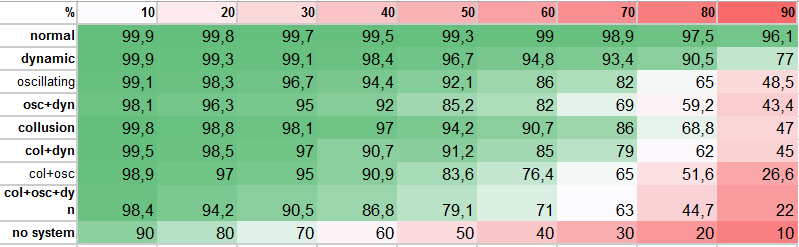
\includegraphics[scale={0.9}]
		{diagrams/table.PNG}
		\label{fig:table.PNG}
	\end{figure}
\begin{table}
\caption{Πίνακας μέσης ικανοποίησης}
\label{tab:avg_sat}
\end{table}

Εποπτικά μπορούμε να το δούμε τα ίδια συμπεράσματα και στο σχήμα \ref{fig:horizontal.PNG}
 
\diagram{Συμπεριφορά δικτύων}{horizontal.PNG}
\newpage
\section{Ταχύτητα σύγκλισης RT-IOT}

Σε αυτήν την ενότητα παρουσιάζεται πόσο γρήγορα (σε αριθμό συναλλαγών) η μέση ικανοποίηση των Εικονικών Οντοτήτων συγκλίνει στην τελική τιμή της. Για καλύτερη εποπτεία το πείραμα έγινε δύο φορές, την πρώτη το ποσοστό τον κακόβουλων οντοτήτων ήταν σε σχετικά φυσιολογικά επίπεδα (30\%), ενώ στο δεύτερο ήταν σε επίπεδα επίθεσης σε ολόκληρο το σύστημα (70\%). 

Παρακάτω είναι τα διαγράμματα και πάλι για διαφορά είδη δικτύων
\diagram{Ταχύτητα σύγκλισης σε δίκτυο με 30\% κακόβουλων οντοτήτων}{30.PNG}



Όπως μπορούμε να παρατηρήσουμε στο πρώτο σχήμα οι τιμές έχουν συγκλίνει από τους πρώτους 100 κύκλους επειδή σχεδόν όλοι βρίσκουν έναν ικανό αριθμό από καλόβουλες εικονικές οντότητες για να παίρνουν την υπηρεσία χωρίς να χρειαστεί να εξερευνήσουν πολύ. Ενδεικτικό είναι ότι από τους 10 πρώτους κύκλους η μέση ικανοποίηση είναι στο 90\% τις τελικής. Το ότι δεν φτάνουν όλα τα δίκτυα στο 100\% έχε να κάνει με το χρόνο που χρειάζονται οι εικονικές οντότητες να εντοπίσουν αλλαγή συμπεριφοράς και να βρουν κάποιον άλλον να πάρουν την υπηρεσία. 

Αντίθετα σε ένα απλό δυναμικό δίκτυο υπάρχει σύγκλιση στο 100\% επειδή στην λίστα φίλων είναι μόνο καλόβουλες εικονικές οντότητες οπότε μόλις βρεθεί κάποιος ανενεργός, ο επόμενος ενεργός εντός της λίστας θα δώσει την υπηρεσία καλά. Η χαμηλότερη ταχύτητα οφείλεται στο ότι πρέπει να συγκεντρώσει κάθε Ε.Ο. έναν αριθμό από φίλους το οποίο την κάνει αρχικά ευάλωτη σε επιθέσεις.

\diagram{Ταχύτητα σύγκλισης σε δίκτυο με 70\% κακόβουλων οντοτήτων}{70.PNG}
Στο δεύτερο σχήμα φαίνεται ότι η σύγκλιση θέλει παραπάνω κύκλους εκτός από την απλή περίπτωση. Αυτό συμβαίνει επειδή είναι δύσκολο να βρεθούν νέοι φίλοι αφού είναι πιθανό η πλατφόρμα να δίνει λάθος συστάσεις οπότε να χρειάζονται αρκετοί κύκλοι για να βρεθεί κάποιος καλός. 


Αυτό χειροτερεύει στην περίπτωση εναλλαγής συμπεριφοράς (osc) επειδή μπορεί μόλις εμπιστευτεί η Ε.Ο. κάποιον, αυτός να το εκμεταλλευτεί αλλάζοντας συμπεριφορά οπότε να χρειαστεί νέος κύκλος ερωτήσεων.
\newpage

\section{Σύγκριση με δημοφιλή συστήματα εμπιστοσύνης - φήμης}
Για να φανεί  πραγματική αξία του συστήματος σε αυτή την ενότητα
συγκρίνεται με τρία από τα επικρατέστερα συστήματα φήμης εμπιστοσύνης σήμερα (Eigentrust \cite{EigenTrust},PeerTrust\cite{PeerTrust},  PowerTrust\cite{PowerTrust}) 
 καθώς και με ένα σχετικά νέο συστήμα, γνωστό ως BTRM(Bio-Inspired Trust and Reputation Model\cite{BTRM})  εφαρμόζει έναν βιλογικό αλγόριθμο γνωστό ώς Ant-Colony System\cite{Dorigo} (ACS).



\subsection{Σύγκριση Μέσης Ικανοποίησης}

Διενεργήθηκαν πειράματα τόσο σε απλά δίκτυα όσο και σε δίκτυα με δυναμική είσοδο κόμβων ή εναλλαγή συμπεριφοράς. Έγιναν μετρήσεις για διάφορα ποσοστά κακόβουλων οντοτήτων (10,30,50,70,90).
\diagramscale{Σύγκριση σε απλό δίκτυο}{normalcmp.PNG}{0.9}
\diagramscale{Σύγκριση σε δίκτυο δυναμικής εισόδου κόμβων}{osccmp.PNG}{0.9}
\diagramscale{Σύγκριση σε δίκτυο δυναμικής συμπεριφοράς }{dyncmp.PNG}{0.9}
\newpage
Όπως φαίνεται λοιπόν από τα διαγράμματα το RT-IOT έχει συγκρίσιμες επιδόσεις ικανοποίησης σε όλα τα δίκτυα παρόλο που έχει σχεδιαστικούς περιορισμούς αφού οι Ε.Ο. δεν έχουν πλήρη εικόνα για την συμπεριφορά των υπολοίπων. Έτσι ο συνδυασμός κεντρικής αρχής και κατανεμημένων τρόπων υπολογισμού εμπιστοσύνης και φήμης οδηγεί σε ένα σύστημα ικανό να διατηρήσει την ικανοποίηση σε πολύ καλά επίπεδα.

\newpage
\subsection{Σύγκριση Κλιμάκωσης}

Όπως είδαμε το RT-IOT παρέχει παρόμοιες επιδόσεις με τα υπόλοιπα συστήματα σε όλους τους τομείς. Η διαφορά του όμως είναι στο σχεδιασμός από την αρχή. Ούτε η εικονικές οντότητες ούτε η πλατφόρμα έχουν πλήρη εικόνα του συστήματος κάτι που προσφέρει ένα τεράστιο πλεονέκτημα στην κλιμάκωση. Στο παρακάτω διάγραμμα φαίνεται πόσο κατάφεραν να κλιμακώσουν τα διάφορα συστήματα εμπιστοσύνης-φήμης στην προσομοίωση.

\diagramscale{Σύγκριση Κλιμάκωσης}{scale.PNG}{0.8}

Όλες οι μετρήσεις έγιναν σε προσωπικό υπολογιστή με Intel Core i7 3630QM και 8GB RAM. Δόθηκε όριο χρόνο 30sec ανά κύκλο συναλλαγών (1 βήμα στην προσομοίωση δηλαδή). Τα αποτελέσματα φαίνονται στο σχήμα \ref{fig:scale.PNG}. Σημειώνουμε πώς το RT-IOT δεν έφτασε τα 30sec/step αλλά μόνο τα 1 sec/step. Το πρόβλημα ήταν πώς δεν ήταν δυνατό να δημιουργηθούν άλλα threads στο σύστημα.

Όπως είναι εμφανές το RT-IOT κατάφερε να τρέξει προσομοίωση με δεκαπλάσιους κόμβους ενώ πιστεύουμε ότι με αρκετή μνήμη θα ήταν \textbf{250x} .

Γενικά παρατηρήθηκε σχεδόν σταθερός χρόνος/Ε.Ο. κάτι που μεταφράζεται σε σταθερό χρόνο ανά Ε.Ο. και γραμμική κλιμάκωση της πλατφόρμας.

\diagramscale{Χρόνος υπολογισμού βήματος ανά Ε.Ο στο RT-IOT}{timepernode.PNG}{0.8}


\chapter{ Επίλογος και Μελλοντικές Επεκτάσεις}\label{ch:conclusion}
\end{large}


\end{document}
